%%%%%%%%%%%%%%%%%%%%%%%%%%%%%%%%%%%%%%%%%%%%%%%%%%%%%
%%%%%%%%%%%%%%%%%% SET UP DOCUMENT - GENERAL STUFF %%%%%%%%%%%%
%%%%%%%%%%%%%%%%%%%%%%%%%%%%%%%%%%%%%%%%%%%%%%%%%%%%%%

\documentclass{beamer}
%%%		beamer modes: handout, 

%%% PACKAGES LOADED IN BY BEAMER
%%%		amsthm %%use noamsthm to suppress loading this -- see p16 of beameruserguide (BUG)
%%%		color - also xcolor is loaded
%%%		enumerate %% loaded in the presentation modes but not in the article mode
%%%		hyperref   %% to pass additional options to beamer use the following class options: \documentclass[hyperref={<list-of-options}]{beamer}
%%%		for HANDOUTS recommended that you use beamer with the document class article
	%%% \documentclass[<options>]{article}
	%%%	\usepackage[<options>]{beamerarticle}
	%%%	--- see the BUG for more details, pp206
	%%%		xcolor - also color is loaded


\mode<presentation>

%\hypersetup{pdfpagemode=FullScreen} % makes your presentation go automatically to full screen


\usetheme{Madrid}
\usecolortheme{beaver} %crane fly wolverine 

%\useoutertheme[subsection=false]{smoothbars}

\useinnertheme{rectangles}

%\setbeamercovered{transparent}

%%%%%%%%%%%%%%%%%%%%%%%%%%%%%%%%%%%%%%%%%%%%%%%%%%%
%%%		OTHER PACKAGES LOADED IN EVERYTIME	%%%%%%%%%%%
%%%%%%%%%%%%%%%%%%%%%%%%%%%%%%%%%%%%%%%%%%%%%%%%%%%%%

\usepackage{graphicx} % Defines \includegraphics*

\usepackage[latin1]{inputenc}

\usepackage{times}
\usepackage[T1]{fontenc}

\usepackage{pifont} %for dingbat style things such as ARROWS, see the ``symbol-letter guide'' in my Guides folder for LaTeX

% Or whatever. Note that the encoding and the font should match. If T1
% does not look nice, try deleting the line with the fontenc.

\usepackage[absolute,overlay]{textpos}
%%%		beamer automatically installs a white background behind everything, unless you install a different background template. Because of this, you must use the overlay option when using textpos, so that it will place boxes in front of everything. Alternatively, you can install an empty background template, but this may result in an incorrect display in certain situtations with older versions of the Acrobat Reader.


\usepackage{url} % Typeset URLs and e-mail addresses

\usepackage{geometry} %\usepackage{geometry}
%\usepackage{movie15}

%\usepackage{hyperref}

\usepackage{multimedia}

\usepackage{setspace}
%\usepackage{enumitem}
\usepackage{expdlist}
\usepackage{tikz}


\xdefinecolor{darkgreen}{rgb}{0,0.35,0}
\definecolor{wdgRed}{rgb}{.6,0,0}

%%%%%%%%%%%%%%%%%%%%%%%%%%%%%%%%%%%%%%%%%%%%%%%%%%%%%
%%%%%%%%%%%%%%%%%% Biblatex APA6 Stuff %%%%%%%%%%%%%%%%%%%%%%%%
%%%%%%%%%%%%%%%%%%%%%%%%%%%%%%%%%%%%%%%%%%%%%%%%%%%%%%
\usepackage[american]{babel}
\usepackage{csquotes}
\usepackage[style=apa,backend=biber]{biblatex}
\DeclareLanguageMapping{american}{american-apa}

\addbibresource{/Users/GrayMatter/Library/texmf/tex/wdg_master_Bib.bib} %my default biblatex file

\setlength{\bibhang}{1.5em}  %%% adjusts the hanging indent size


%%% PATHNAME FOR LOGO FIGURES
%% /Users/GrayMatter/Library/texmf/tex/zLogoFigs

\usepackage[yyyymmdd]{datetime}

\usepackage{verbatim}

%%%%%%%%%%%%%%%%%%%%%%%%%%%%%%%%
%%%%	BEAMER SETUPS
%%%%%%%%%%%%%%%%%%%%%%%%%%%%%%%
\AtBeginSection[] % Do nothing for \section*
{
	\begin{frame}<beamer>
		\frametitle{Outline}
		\tableofcontents[currentsection]
	\end{frame}
}

\AtBeginSubsection[]
{
 \begin{frame}<beamer>{Outline}
 \tableofcontents[currentsection,currentsubsection]
 \end{frame}
}

%these commands can make the cell entries ragged right 
%\newcommand{\rr}{\raggedright}
%\newcommand{\tn}{\tabularnewline}

%\titlegraphic{\includegraphics[width=\textwidth,height=.5\textheight]{someimage}}

% If you have a file called "university-logo-filename.xxx", where xxx
% is a graphic format that can be processed by latex or pdflatex,
% resp., then you can add a logo as follows:

\pgfdeclareimage[height=1cm]{university-logo}{/Users/GrayMatter/Library/texmf/tex/zLogoFigs/CWL-s.pdf} %[height=0.5cm]
\logo{\pgfuseimage{university-logo}}

% If you wish to uncover everything in a step-wise fashion, uncomment
% the following command: 

%\beamerdefaultoverlayspecification{<+->}

%%%%%%%%%%%%%%%%%%%%%%%%%%%%%%%%%%%%%%%%%%%%%%%%%%%%%
%%%%%%%%%%%%%%%%%% Title Page Info %%%%%%%%%%%%%%%%%%%%%%%%%%%
%%%%%%%%%%%%%%%%%%%%%%%%%%%%%%%%%%%%%%%%%%%%%%%%%%%%%%

\title[Cognitive Workload] % (optional, use only with long paper titles)
{Contributions of Body-Bound \& Brain-Bound Resources, and Control Processes to Cognitive Workload}


\author[Gray \& Ralph]%
{Wayne D. Gray\inst{1,}\inst{2,}\inst{3} \& Jason Ralph\inst{1}} % (optional, use only with lots of authors)
% - Give the names in the same order as the appear in the paper.
% - Use the \inst{?} command only if the authors have different affiliations.

\institute[RPI, MPIB, Humboldt] % (optional, but mostly needed)
{
 \inst{1}
 Cognitive Science Department, Rensselaer Polytechnic Institute\\
 \inst{2}
 Alexander von Humboldt Stiftung/Foundation\\
 \inst{3}
 Center for Adaptive Behaviour and Cognition, Max Planck Institute for Human Development
 }
% - Use the \inst command only if there are several affiliations.
% - Keep it simple, no one is interested in your street address.

\date[\today] % (optional, should be abbreviation of conference name)
{Talk Presented at UCL on 2012-03Mar-07}
% - Either use conference name or its abbreviation.
% - Not really informative to the audience, more for people (including yourself) who are reading the slides online

%\subject{<>}
% This is only inserted into the PDF information catalog. Can be left
% out. 


\begin{comment}
\begin{frame}
	\frametitle{}
	\begin{itemize}
		\item
	\end{itemize}
\end{frame}
\end{comment}


%%%%%%%%%%%%%%%%%%%%%%%%%%%%%%%%%%%%%%%%%%%%%%%%%%%%%
%%%%%%%%%%%%%%%%%% BEGIN DOCUMENT HERE %%%%%%%%%%%%%%%%%%%%%
%%%%%%%%%%%%%%%%%%%%%%%%%%%%%%%%%%%%%%%%%%%%%%%%%%%%%%

\begin{document}

\begin{frame}
 \titlepage

\end{frame}

\begin{frame}
	\frametitle{THANKS TO OUR SPONSORS!}
	  \begin{textblock}{3}(.5,1.5)	
  		{\includegraphics[scale=1]{/Users/GrayMatter/Library/texmf/tex/zLogoFigs/AvH-Logo}}
    	   \end{textblock} 
   	  \begin{textblock}{3}(5.5,7)	
  		{\includegraphics[scale=.15]{/Users/GrayMatter/Library/texmf/tex/zLogoFigs/ONR-150dpi}}
    	   \end{textblock} 
	    \begin{textblock}{3}(10,10)	
  		{\includegraphics[scale=.5]{/Users/GrayMatter/Library/texmf/tex/zLogoFigs/minerva}}
    	   \end{textblock} 
\end{frame}

\begin{frame}[basicstyle=\small]
	\frametitle{OUTLINE}
 	 \tableofcontents   %[pausesections]
  % You might wish to add the option [pausesections]
\end{frame}

%% motivation				motivation
\section{Motivation}
%% motivation				motivation
\subsection{Orientation}

 \begin{frame}
	\frametitle{ORIENTATION}
Cognitive workload is a Pasteur's Quadrant \parencite{stokes97} type of problem:
		\begin{itemize}
			\item An important applied problem the solution of which requires development of basic theory in control of cognition
		\end{itemize}

	\begin{textblock}{9}(1,13)
		\begin{alertblock}{}
			\tiny{\fullcite{stokes97}}
		\end{alertblock}
	\end{textblock}

\end{frame}

\begin{frame}
	\frametitle{BUT FIRST\dots}
	\begin{itemize}
		\item The talk I might have given yesterday but did not\dots
	\end{itemize}
		\begin{center}
		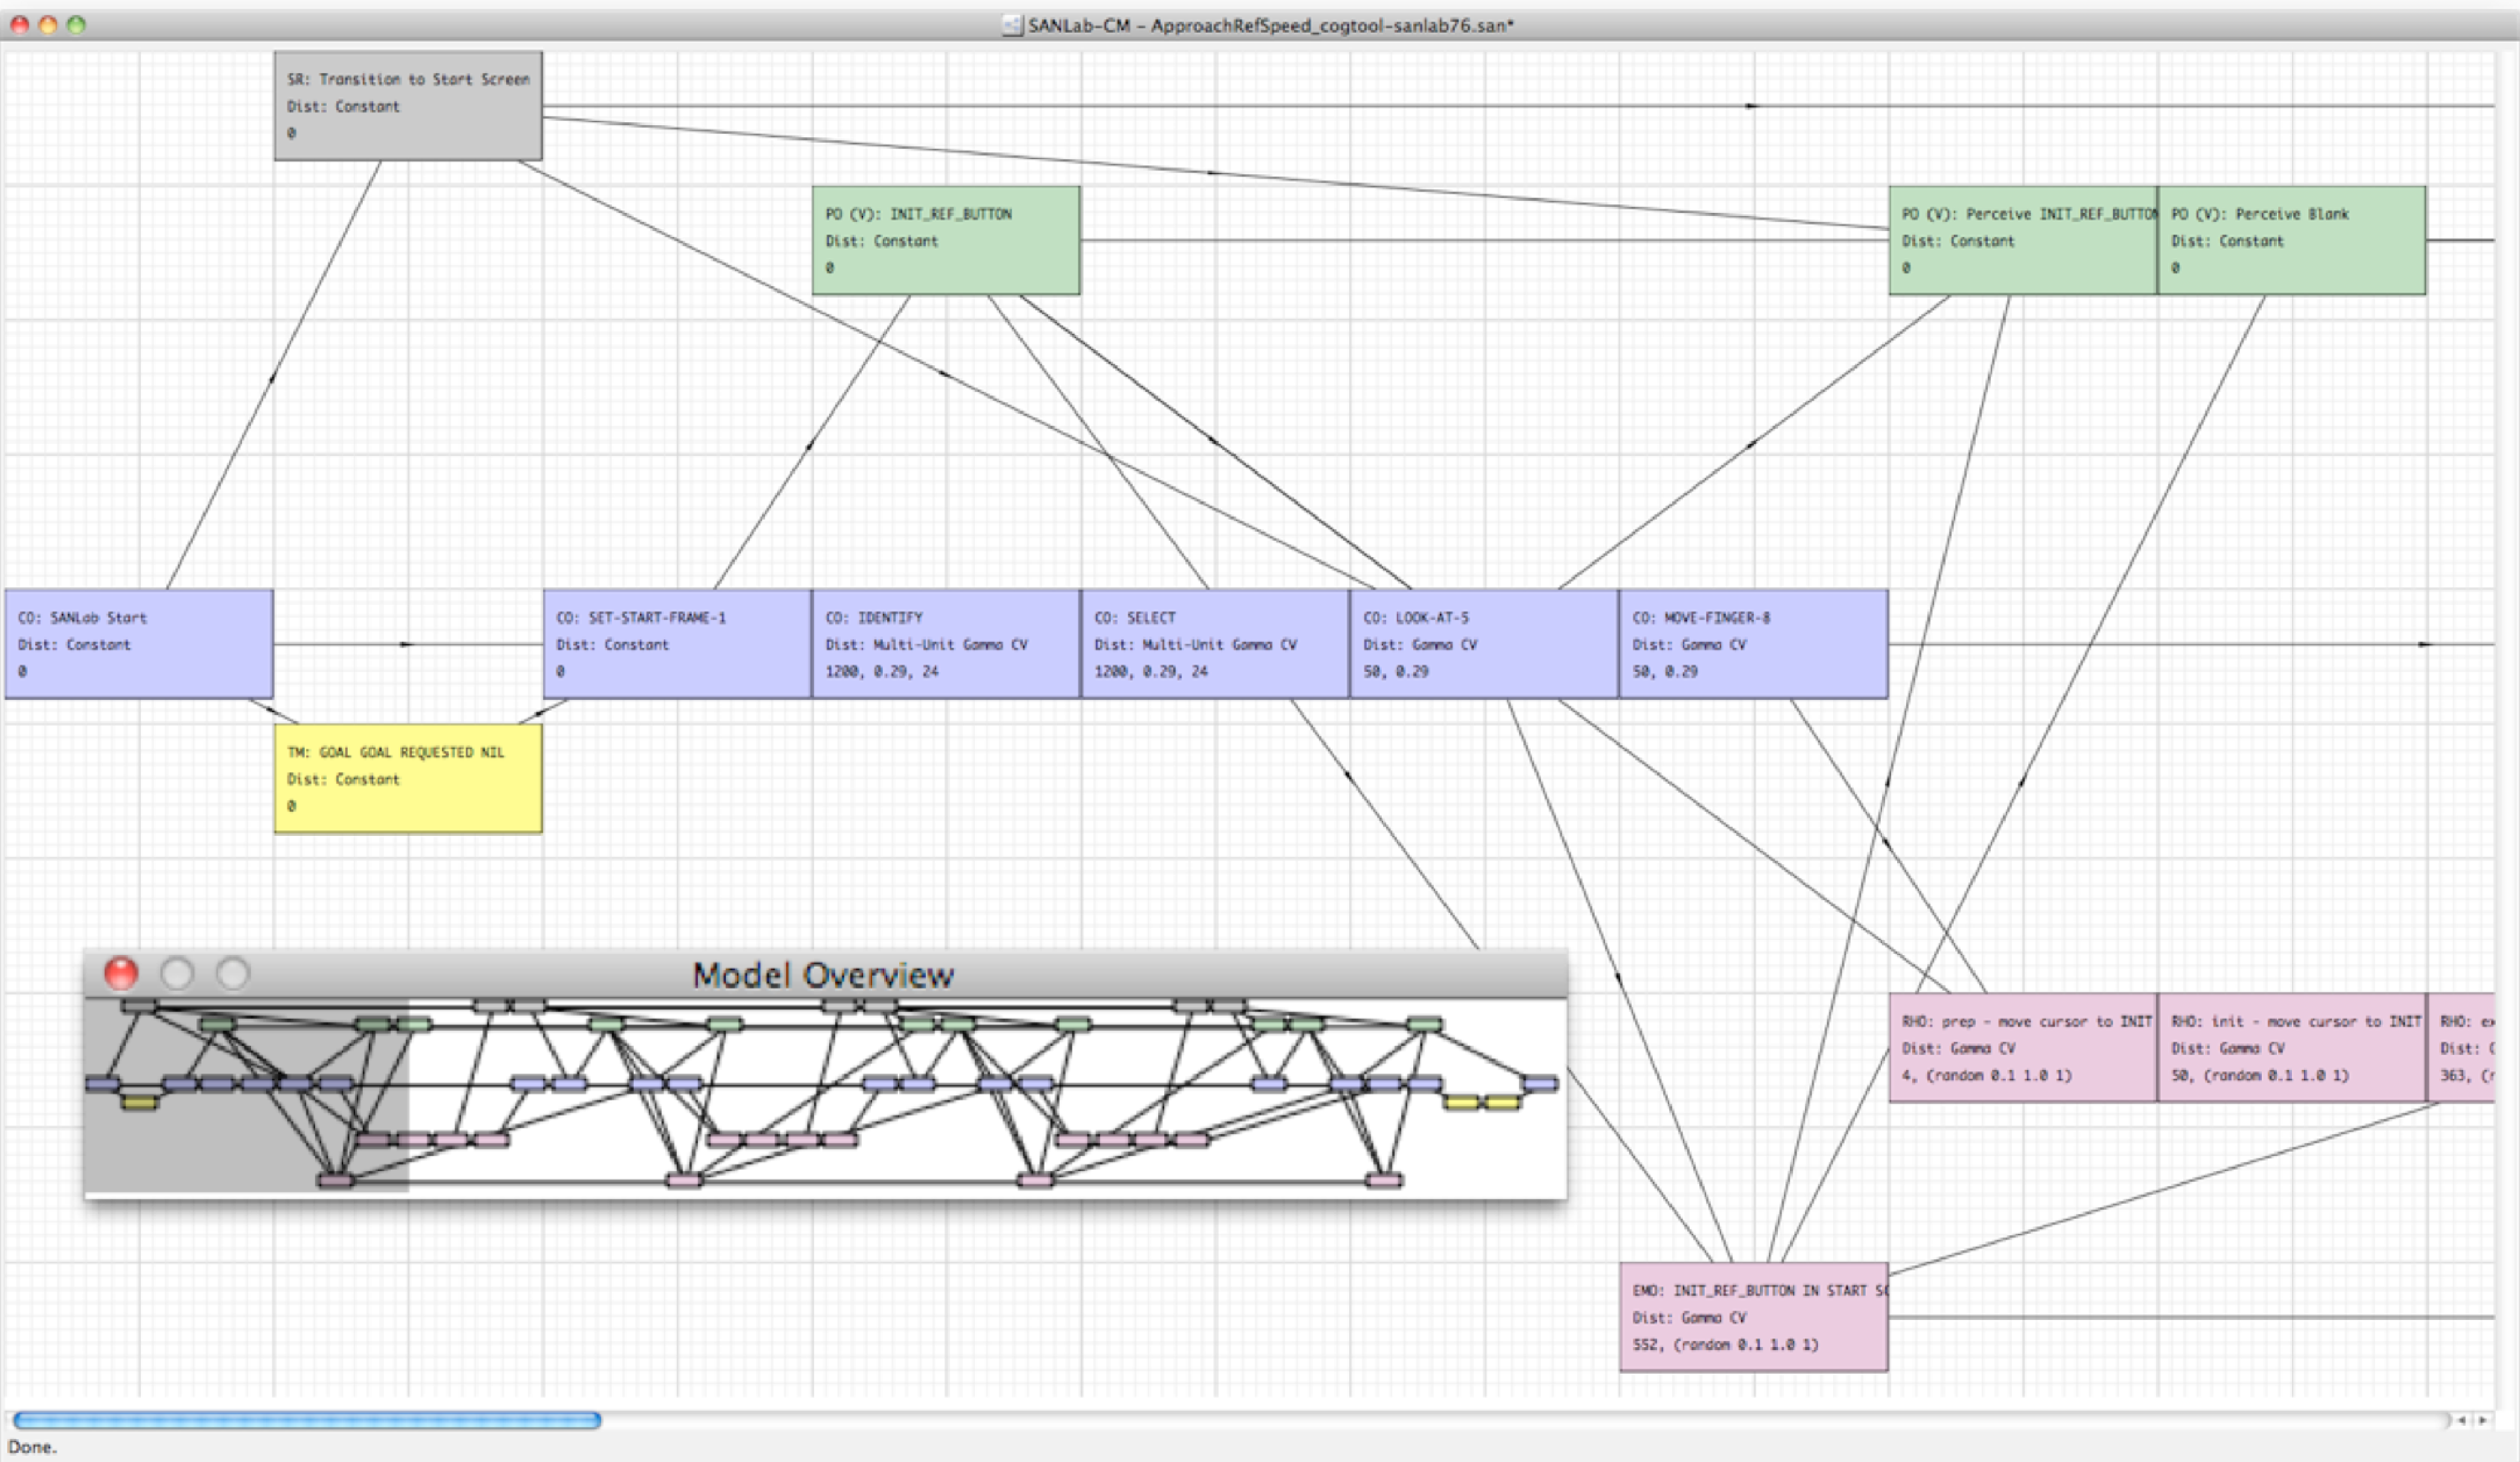
\includegraphics[width=.75\textwidth]{../zNvBkFigs/fig4-SL}
	\end{center}
\end{frame}

\begin{frame}
	\frametitle{BUT FIRST\dots}
	\begin{itemize}
		\item The talk I might have given yesterday but did not\dots
	\end{itemize}
		\begin{center}
		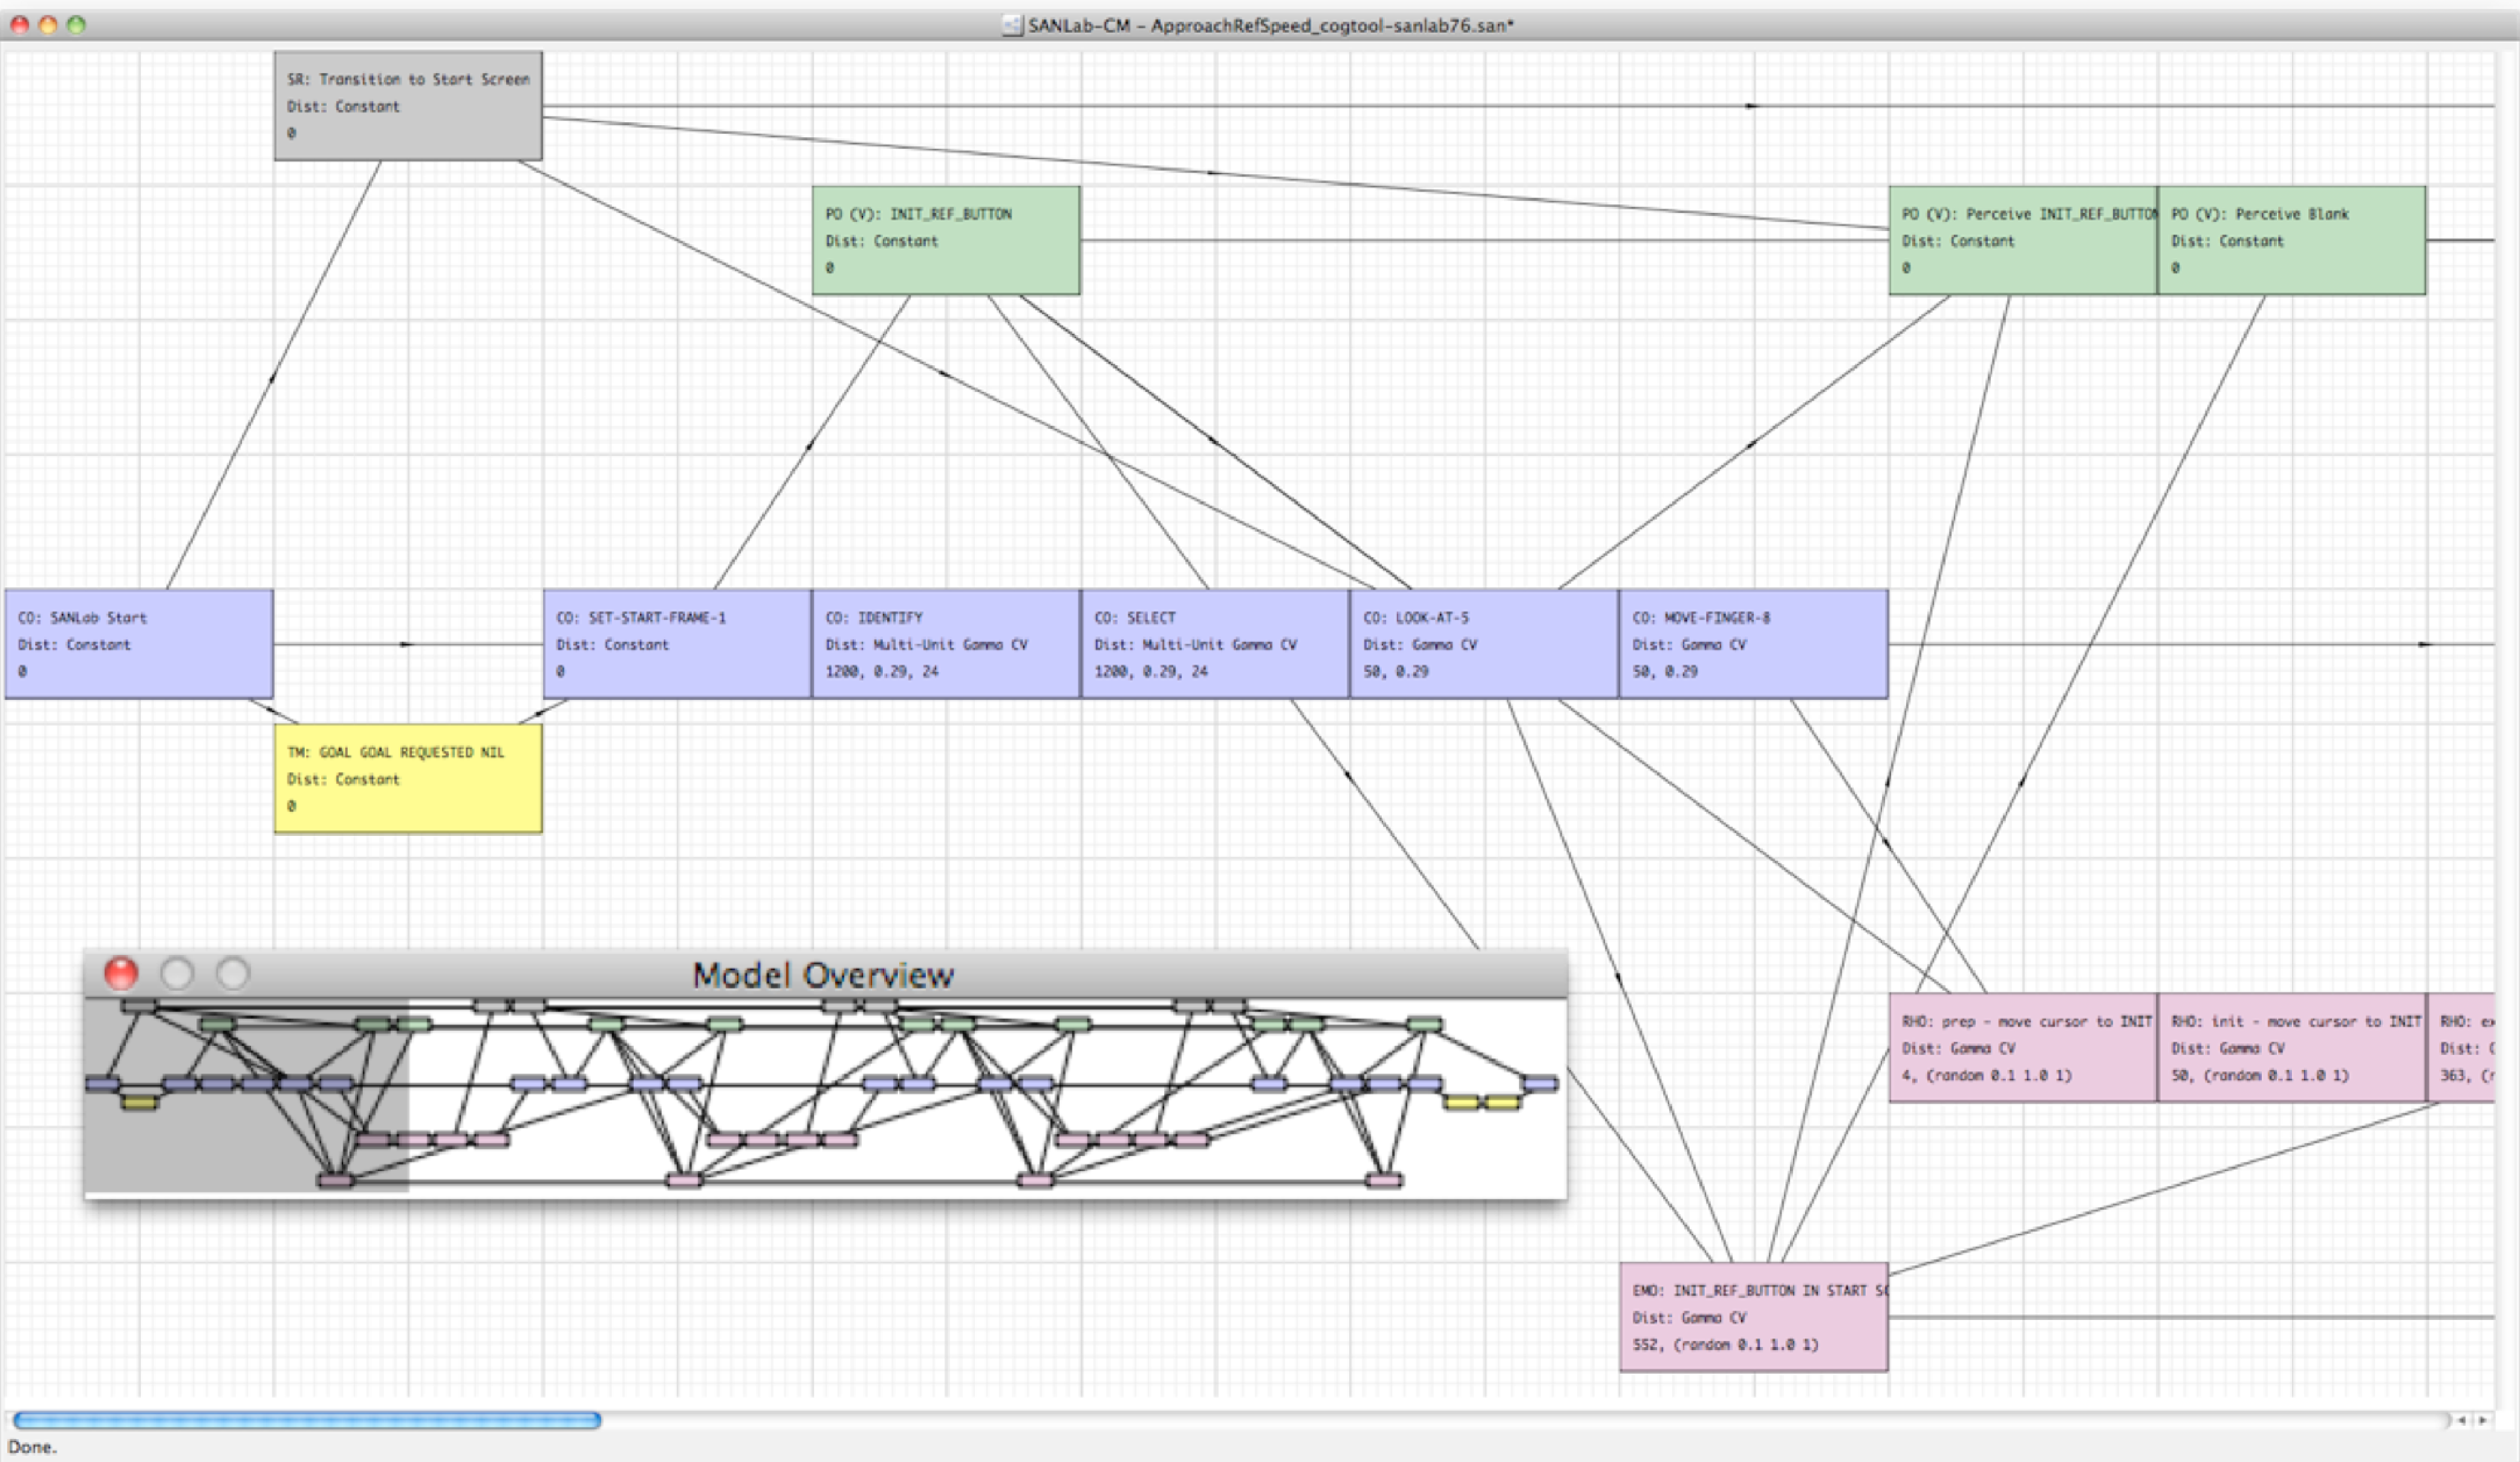
\includegraphics[width=.75\textwidth]{../zNvBkFigs/fig4-SL}
	\end{center}
	\begin{textblock}{3}(5.5,7)	
  		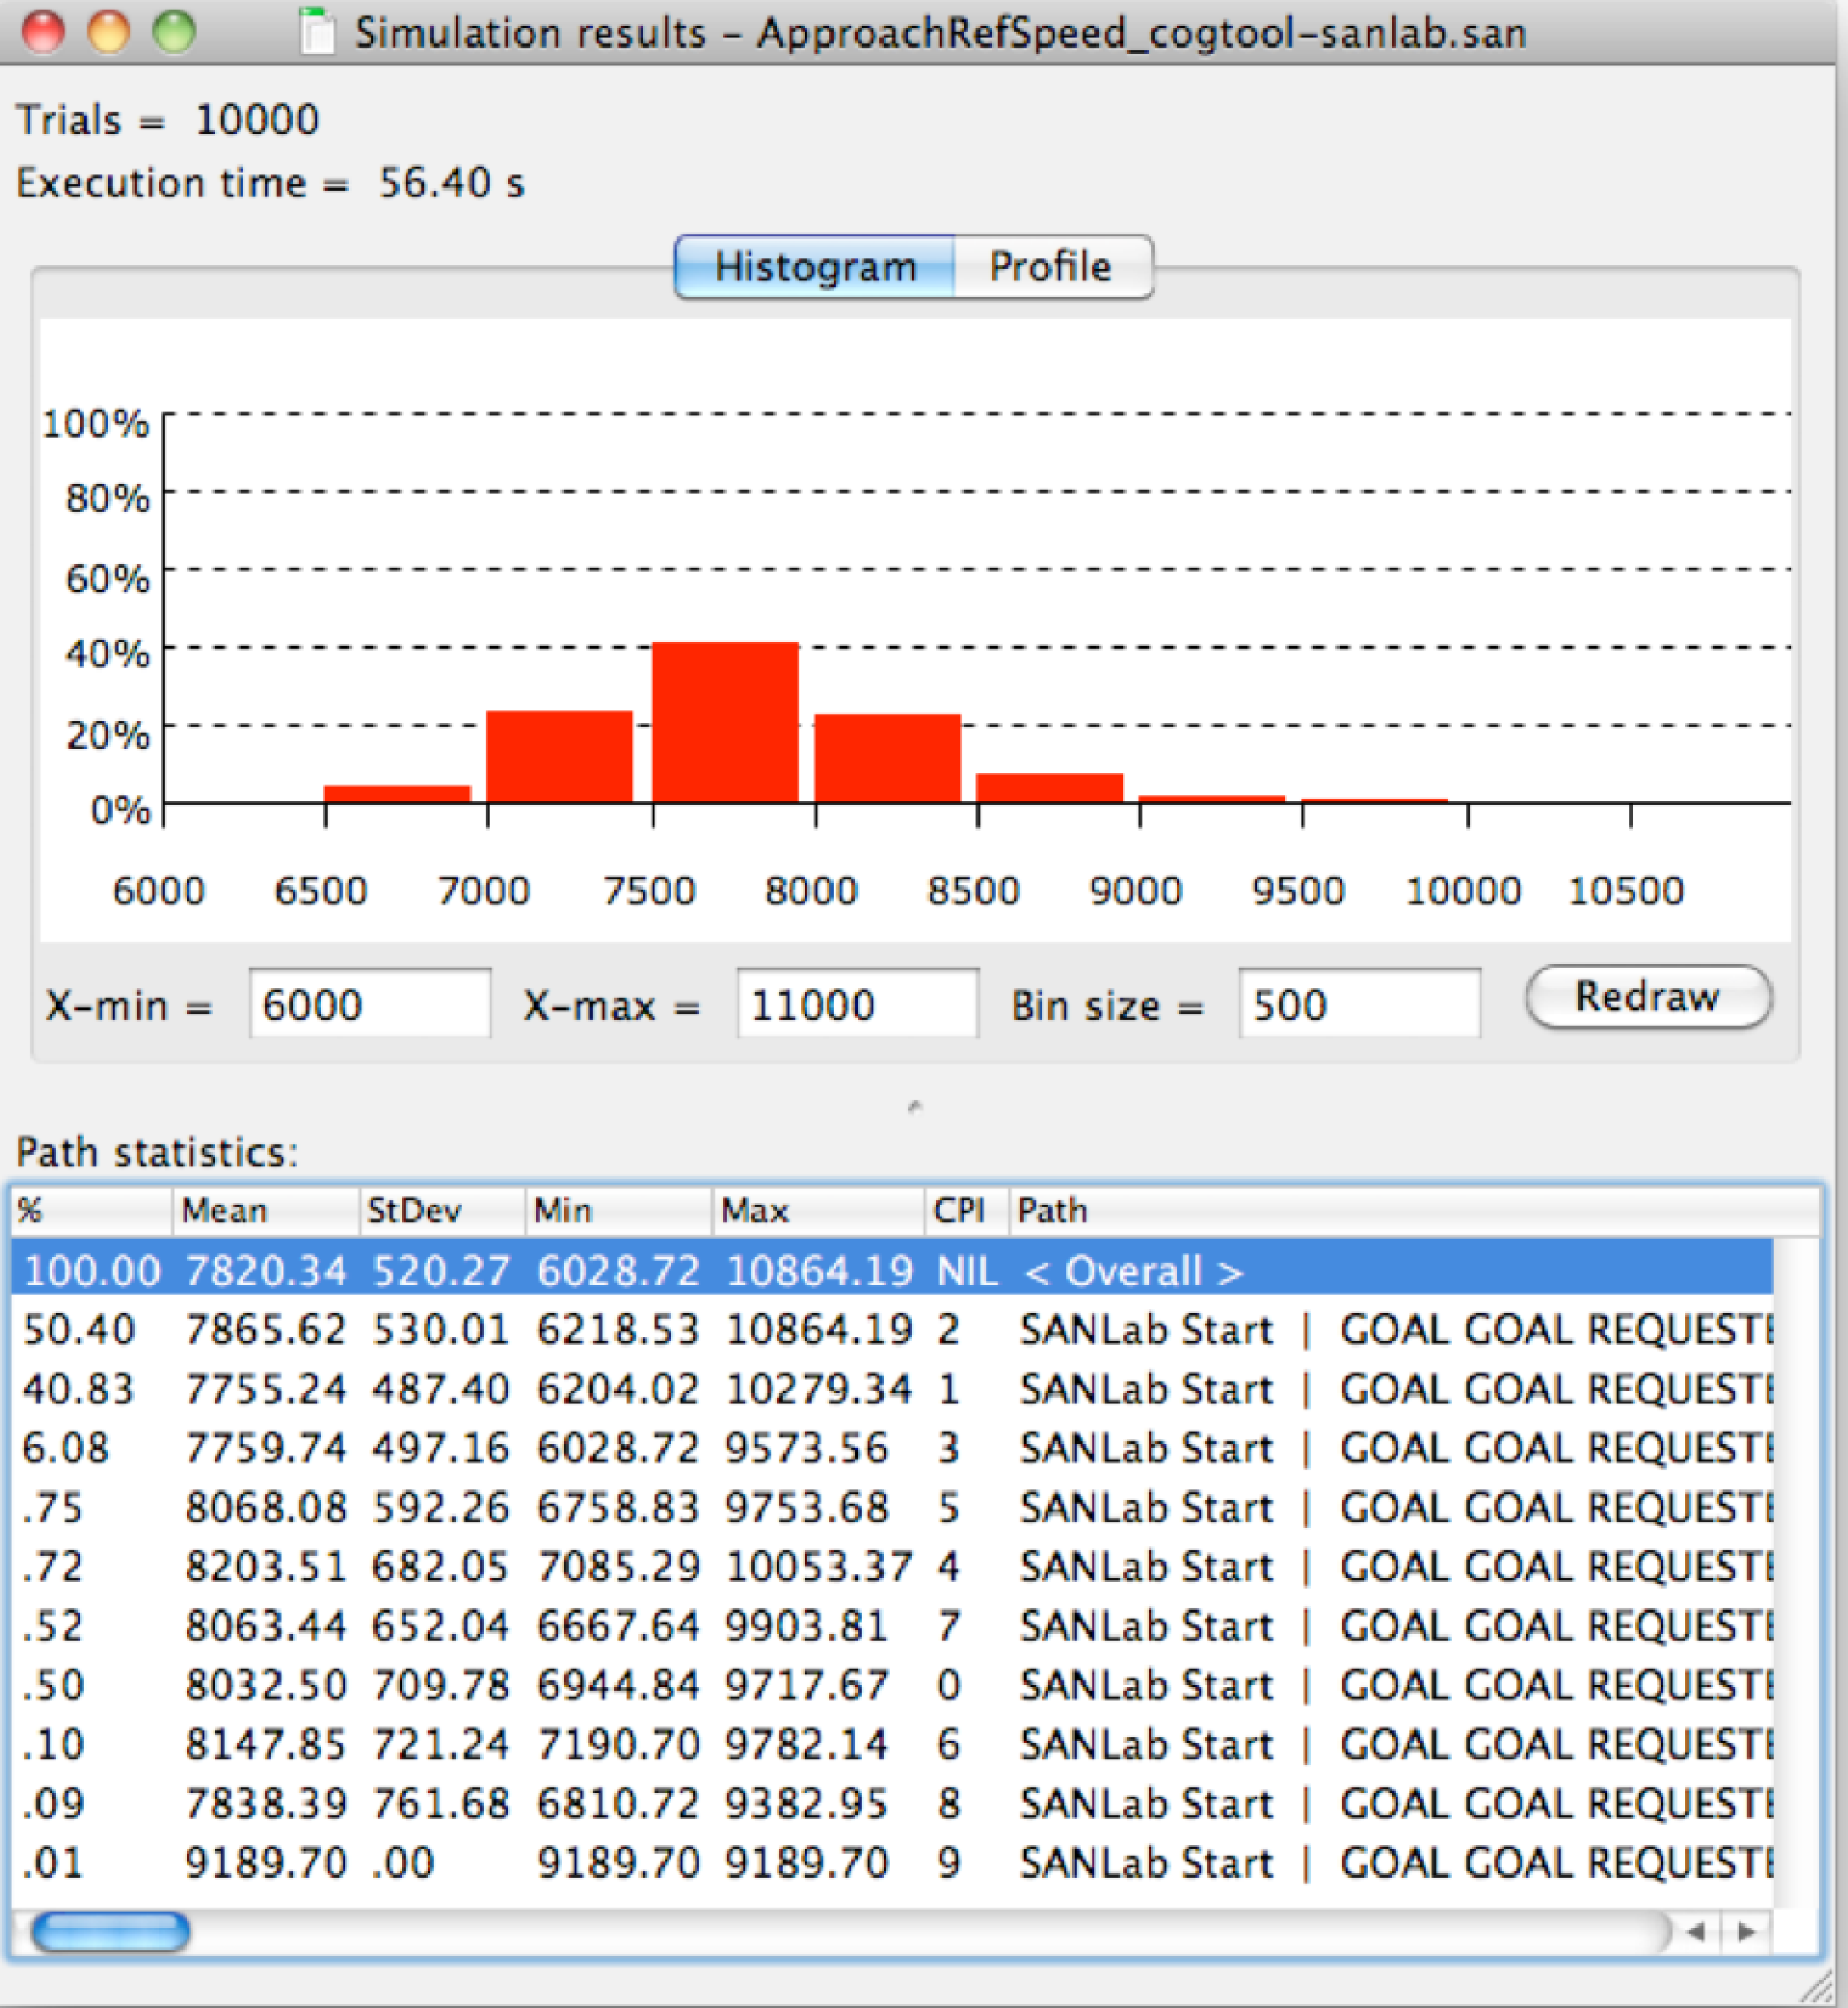
\includegraphics[width=.75\textwidth]{../zNvBkFigs/fig5-SLhist}
    	   \end{textblock}
\end{frame}


\begin{frame}
	\frametitle{THE CHALLENGE}
Solving this problem will not be business-as-usual for the cognitive research community
	\begin{itemize}
			\item The scope of the problem may result in a different approach to theory development than many cognitive scientists favor
			\item A broader consideration of the interactions among cognition, perception, and action is required
			\begin{itemize}
				\item Echoes the distinction made by EPIC, ``to give the perceptual and motor mechanisms equal status with cognition in accounting for human performance,'' \nptextcite{km97}
			\end{itemize}
			\pause
			\item A broader take on modeling is required as well. The need to model entire tasks, not just the bits that are simple to model \parencite{erik08pr.article,newell73chptr}
		\end{itemize}

\end{frame}

 \begin{frame}
	\frametitle{WHY COGNITIVE WORKLOAD IS IMPORTANT}
	The need for theory-based applications:
	\begin{itemize}
		\item Real: Performance decrements due to cognitive overload are real and well documented
		\item State-of-the-Art is an Art: Going beyond \emph{intuitive} solutions of the occasionally gifted designer will require basic research into the control of cognitive systems
		\item Who? The push for theories of cognitive workload has been driven primarily by educational and human factors researcher, often with very little direct input from the basic research community
	\end{itemize}
\end{frame}

%% Review and Critique
\subsection{Review and Critique of Contemporary Theory of Workload}
%% Review and Critique

\begin{frame}[label=4flaws]
	\frametitle{WORKLOAD, COGNITIVE WORKLOAD, \& COGNITIVE CONTROL}
	Current approaches to workload used by the human factors community share one or more flaws:
	\begin{enumerate}
		\item They offer an outcome-based not a process-based approach to workload
		\item They treat workload as a single construct that applies over the full scope of human behavior
		\item They do not distinguish between body-bound or brain-bound resource limits
		\item They do mention cognitive control and they certainly do not distinguish between resources limits in control per se versus the role that control plays in selecting different \alert{microprocedures}\footnote[frame]{AKA \emph{interactive routines, microstrategies}} to accomplish a given task (as per \nptextcite{gray06pr}).
	\end{enumerate}
	\vspace{.7cm}
\end{frame}

\begin{frame}
	\frametitle{NON-COGNITIVE APPROACHES TO MENTAL WORKLOAD}
	A disparate dichotomy of questionnaires and psychophysiological data					\begin{itemize} 
		\item Questionnaire Approaches:
		\begin{itemize}
			\item Define workload as the feeling of working hard (e.g., \nptextcite{averty04,didomenico08,hart88})
		\end{itemize}
		\item Electrophysiological Approaches
		\begin{itemize}
			\item Define it in terms of performance deficits
		\end{itemize}
		\item These approaches appear to be polar opposites but both share the four flaws listed earlier.
	\end{itemize}
\end{frame}

\begin{frame}
	\frametitle{COGNITIVE APPROACHES TO MENTAL WORKLOAD}
On the plus side they address the first two complaints; namely,
	\begin{enumerate}
		\item They offer an outcome-based not a process-based approach to workload
		\item They tend to be focused on the unit task level of analysis (3-30s), though this is not an explicit focus
	\pause
  \listpart{However, they don't do so well on these:}  %%%courtesy of the expdlist package
		\item They do not distinguish between body-bound or brain-bound resource limits
		\item They do not distinguish between resources limits in cognitive control versus the role that control resources play in strategically structuring and interleaving body-bound and other brain-bound resources.
	\end{enumerate}
	\vspace{.7cm}

\end{frame}

\begin{frame}
	\frametitle{COGNITIVE APPROACHES}
	The two best examples of cognitive approaches to workload are:
	\begin{itemize}
		\item Sweller's \emph{Cognitive Load Theory} (CLT) \parencite{chandler96acp,leahy03,leahy11,vanmerri05,sweller88}
		\begin{itemize}
			\item An important influence in the Education community
		\end{itemize}
		\pause
	\listpart{\&}
		\item Wicken's \emph{Multiple Resource Theory} (MRT) \parencite{wickens81,wickens92book,wickens02}
		\begin{itemize}
			\item An important influence in the Human Factors community
		\end{itemize}
	\end{itemize}
\pause
Due to their domains, Wicken's MRT has had more to do with complex tasks involving a human operator physically interacting with external devices (e.g., Airline Pilots flying planes)


\end{frame}

\begin{frame}
	\frametitle{MULTIPLE RESOURCE THEORY}
	\begin{itemize}
		\item Visual representation of Christopher Wicken's Multiple Resource Theory. Dual tasks are coded by which sections of the cube the tasks require. When more than one task requires the use of a given resource, the theory predicts a performance decrement.
	\end{itemize}
	\begin{center}
		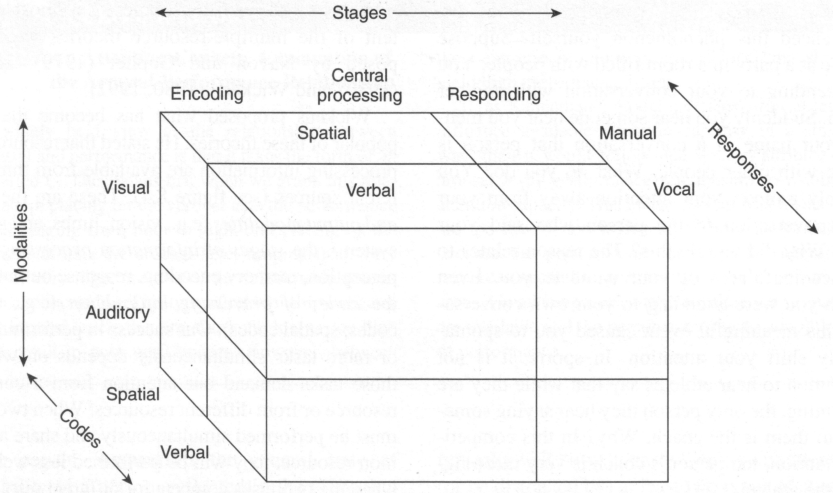
\includegraphics[width=.75\textwidth]{../zNvBkFigs/wickens-mrt}
	\end{center}
\end{frame}

\begin{frame}
	\frametitle{CRITIQUE OF MULTIPLE RESOURCE THEORY}
On the plus side MRT addresses the first two complaints; namely,
	\begin{enumerate}
		\item It offers an outcome-based not a process-based approach to workload
		\item It treats to focus on events that happen with the unit task timeframe (though this focus is not explicit)
	\pause
  \listpart{However, it doesn't do so well on these:}  %%%courtesy of the expdlist package
		\item It does not distinguish between body-bound or brain-bound resource limits
		\item It does not distinguish between resources limits in cognitive control versus the role that control resources play in strategically structuring and interleaving body-bound and other brain-bound resources.
	\end{enumerate}
\end{frame}

%% Our Approach
\subsection{Our Approach}
%% Our Approach

\begin{frame}
	\frametitle{OUR APPROACH TO COGNITIVE WORKLOAD}
Our critique:
	\begin{enumerate}
		\item Current approaches to workload offer an outcome-based not a process-based approach to workload
	\end{enumerate}
	\pause
In contrast, we are:
	\begin{enumerate}
		\item Grounded in process theories of cognition with a computational modeling emphasis \emph{(However, I won't talk about models today.)}
	\end{enumerate}
\end{frame}

\begin{frame}
	\frametitle{OUR APPROACH (2)}
Our critique:
	\begin{enumerate}
		\setcounter{enumi}{1}
		\item Current approaches treat workload as a single construct that applies over the full scope of human behavior
	\end{enumerate}
	\pause
In contrast, we are:
	\begin{enumerate}
		\setcounter{enumi}{1}
		\item Focused on immediate, interactive behavior and the cognitive-perceptual-motor phenomenon that emerge around the 1/3 to 3s level of analysis \emph{(i.e., microprocedures)}
		\begin{itemize}
			\item Our claim is that this level of analysis is required to understand behavior at the Unit Task level \parencite{cmn1983} (3-30s).
		\end{itemize}
	\end{enumerate}
\end{frame}


\begin{frame}
	\frametitle{OUR APPROACH (3)}
Our critique:
	\begin{enumerate}
		\setcounter{enumi}{2}
		\item Current approaches do not distinguish between body-bound or brain-bound resource limits
	\end{enumerate}
\pause
Our approach: 
	\begin{enumerate}
		\setcounter{enumi}{2}
		\item Broadly congruent with discussions of embodied cognition \parencite{clark08,rupert10,km97} as those discussions concern immediate interactive behavior
	\end{enumerate}
\end{frame}

\begin{frame}
	\frametitle{OUR APPROACH (4)}
Our critique:
	\begin{enumerate}
		\setcounter{enumi}{3}
		\item Current approaches do not distinguish between resources limits in cognitive control versus the role that control resources play in strategically structuring and interleaving body-bound and other brain-bound resources.
	\end{enumerate}
\pause
Our approach: 
	\begin{enumerate}
		\setcounter{enumi}{3}
		\item \alert{Milliseconds Matter!} We build on our prior work with the \emph{Soft Constraints Hypothesis} \parencite{gray06pr} which shows shifts in \emph{microprocedures} which reflect local optimization of effort
	\end{enumerate}
	\begin{itemize}
			\item In the work presented today we will be open-minded about whether our data show \alert{resource limits} or \alert{shifts in microstrategies} due to local optimization of efficiencies - as per the \emph{soft constraints hypothesis}.
		\end{itemize}

\end{frame}

\begin{frame}
	%\renewcommand{\labelenumi}{\Alph{enumi}}
	\frametitle{CONTROL OF COGNITION}
	\begin{itemize}
		\item A complete theory of cognitive workload must consider: 
		\begin{enumerate}[\Alph{enumi}]
			\item Body-bound resources which enable us to interact with and gain information from the world
			\item Brain-bound resources that process visual information, produce motor plans, retrieve information from memory, and so on
		\end{enumerate}
		\pause
		\item In addition, cognitive control is itself a resource that is limited and a complete theory of cognitive workload must consider
		\begin{enumerate}[\Alph{enumi}]
			\setcounter{enumi}{2}
			\item Processing limits and resources constraints inherent to the cognitive controller
		\end{enumerate}
		\pause
		\item While we do not yet have a \emph{complete theory}, we refer to our work on cognitive workload as the \emph{Functional Resource Framework}
	\end{itemize}

\end{frame}

\begin{comment}

		\item Adopt the distinction between proactive and reactive cognitive control  \parencite{braver07book.chptr,braver12tics.paper} 
		\begin{itemize}
			\item Proactive control requires a workload intensive `active maintenance of goal-relevant information'
			\item Reactive control is engaged `only as needed', `after, rather than before the occurrence of some imperative event.' 
		\end{itemize}
		\pause

\begin{frame}
	\frametitle{}
	\begin{itemize}
		\item
	\end{itemize}
\end{frame}
\end{comment}



%%% INTRODUCING NAVBACK
\section{The NavBack Paradigm}
%%% INTRODUCTING NAVBACK

\begin{frame}
	\frametitle{NavBack}
	\begin{itemize}
		\item Navigation paradigm that simulates the approximate level of complexity of many laboratory tasks used by Sweller and Wickens' in developing their theories of workload
		\item Dual tasks
		\begin{itemize}
			\item Tracking task -- Jitter
			\item Memory task -- n-back
		\end{itemize}
	\end{itemize}
\end{frame}

\begin{frame} 
	\frametitle{NavBack}
	\begin{center}
		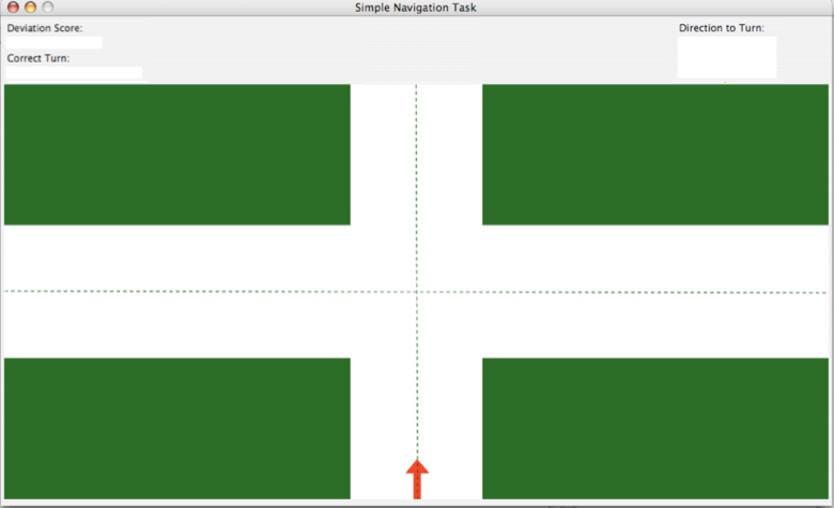
\includegraphics[width=.75\textwidth]{../zNvBkFigs/NavBack}
	\end{center}


\end{frame}

\begin{frame} 
	\frametitle{Directions were given at one of 3 random intervals while arrow was in a city-block corridor}
	\begin{center}
		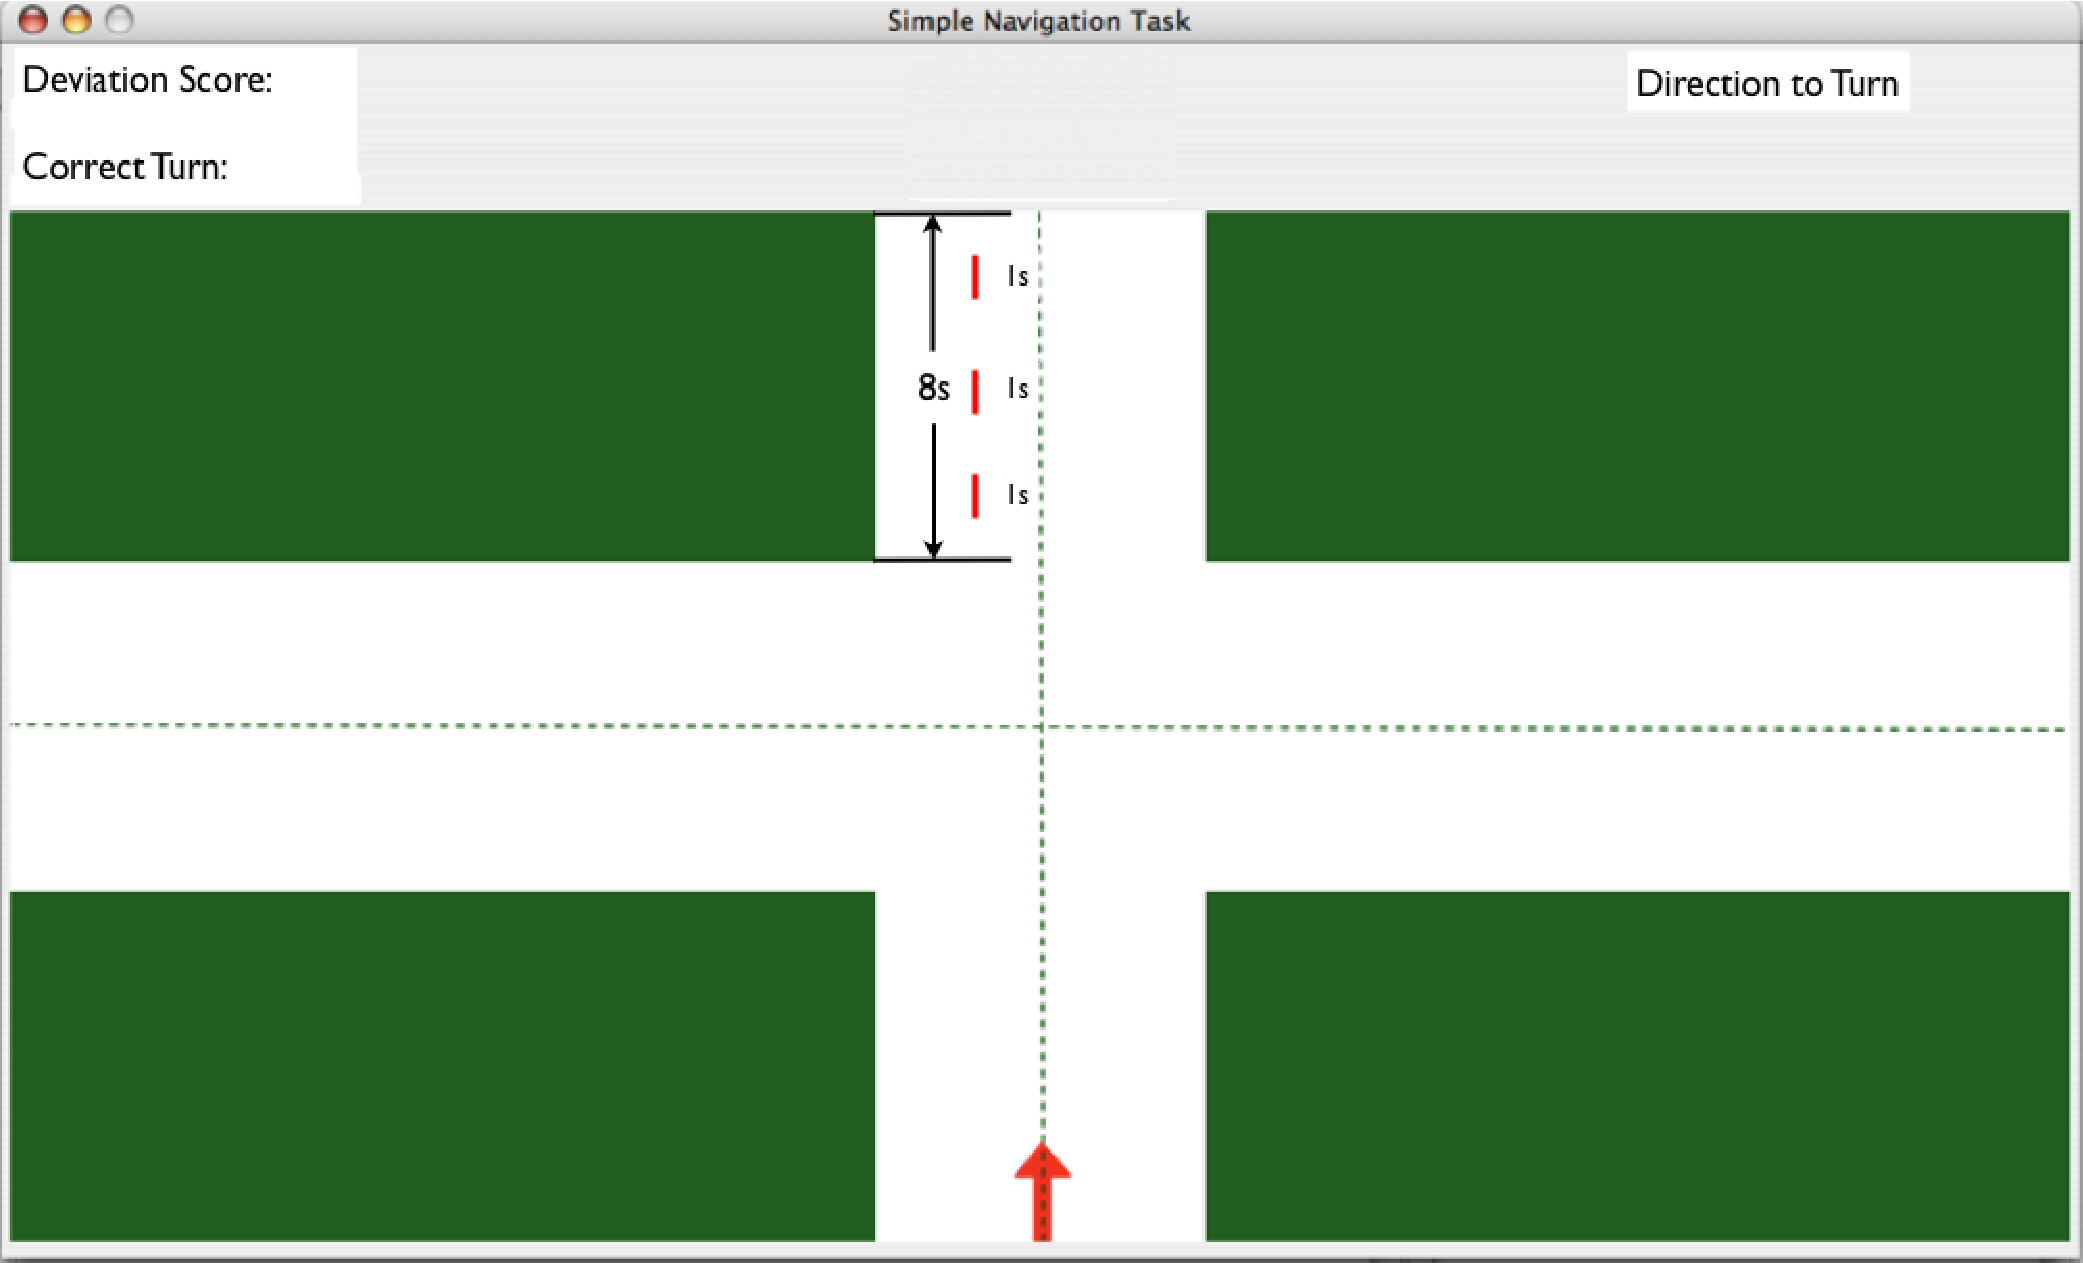
\includegraphics[width=.75\textwidth]{../zNvBkFigs/NavBack-w-intrvls}
	\end{center}
	\only<2>{\begin{textblock}{3}(7.6,7.8)	
  		
\includegraphics[scale=.25]{../zNvBkFigs/red-arrow}
    	 \end{textblock}}
	 \only<3>{\begin{textblock}{3}(7.6,7)	
  		
\includegraphics[scale=.25]{../zNvBkFigs/red-arrow}
    	 \end{textblock} }
	\only<4>{\begin{textblock}{3}(7.6,6.2)	
  		
\includegraphics[scale=.25]{../zNvBkFigs/red-arrow}
    	 \end{textblock} }
 \end{frame}



\begin{frame} 
	\frametitle{TIME COURSE OF AN EPISODE CYCLE}
	\begin{figure}
	\centering
	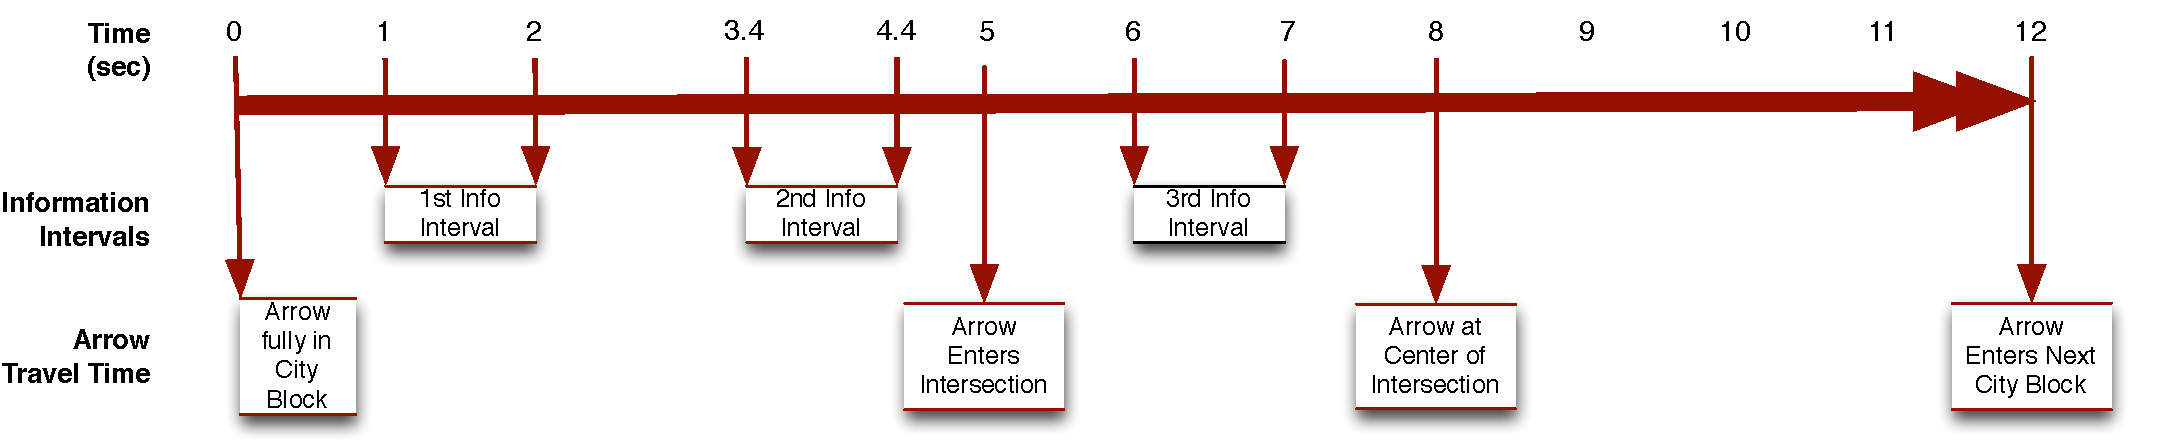
\includegraphics[width=\textwidth]{../zNvBkFigs/Intrsctn-Epsd-Cycle-120305}
	\label{Epsd-Cycle}
	\end{figure}

	\begin{itemize}
		\item 	Cycle begins with the arrow fully in the new City Block
		\item For left and right turns, the cycle ends when the turn begins
		\item For forwards, although movement is continuous, for data collection purposes the episode cycle ends when the tip of the arrow reaches the center of the intersection
	\end{itemize} 
\end{frame}

%%% EXPERIMENT 1
\subsection{Experiment 1}
%%% EXPERIMENT 1


\begin{frame} 
	\frametitle{EXPERIMENT 1}
	\begin{itemize}
		\item  Two conditions: varied in how the instructions were delivered
		\item The tracking task in both conditions required the visual modality
		\begin{itemize}
			\item  Visual: Instructions appeared in the direction box at one of three time periods selected at random (single modality)
			\item Auditory: Instructions read using a standard Mac voice beginning at one of the three time periods (as per the Visual condition) (mixed modlaity)
		\end{itemize}
	\pause
	\item Both Wicken's MRT and our FRF would predict that that visual condition would do worse than the auditory
	\item However, whereas both approaches focus on brain-bound issues, the FRF extends its focus to body-bound and control issues
	\item This broader focus leads us to look for differences in predicted outcomes at a more microlevel
	\end{itemize} 
 \end{frame}

\begin{frame}
	\frametitle{EXPERIMENT 1 - UNSURPRISING RESULT \#1}
	\begin{itemize}
		\item Found significant affect of modality on Turn Accuracy
	\end{itemize}
	\begin{figure}
		\centering
		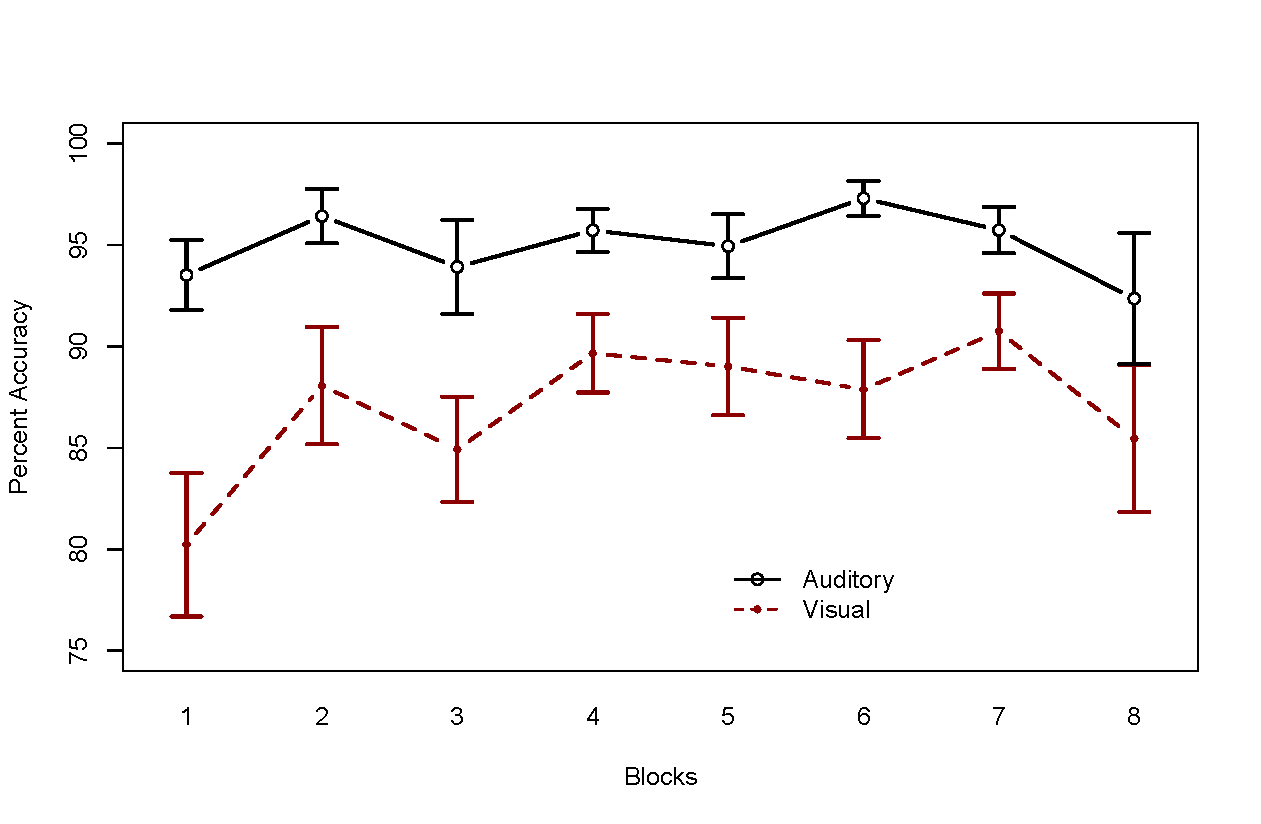
\includegraphics[width=.8\textwidth]{../zNvBkFigs/Rplot_E1_acc_CondByBlks}
		\begin{itemize}
			\item Main effect of condition, no interactions
		\end{itemize}
	\end{figure}
\end{frame}

\begin{frame}
	\frametitle{EXPERIMENT 1 - UNSURPRISING RESULT \#2}
	\begin{itemize}
		\item Found significant affect of modality on Jitter accuracy (mixed aud/vis > pure visual)
		\item No significant differences involving block or its interactions
		\pause
		\item However, the significant interaction of condition by direction interval caused us to examine the data more closely
	\end{itemize}
\end{frame}

\begin{frame} 
	\frametitle{E1 RESULTS: Jitter by Condition}
	Lower scores are better!
	\begin{figure}
		\centering
		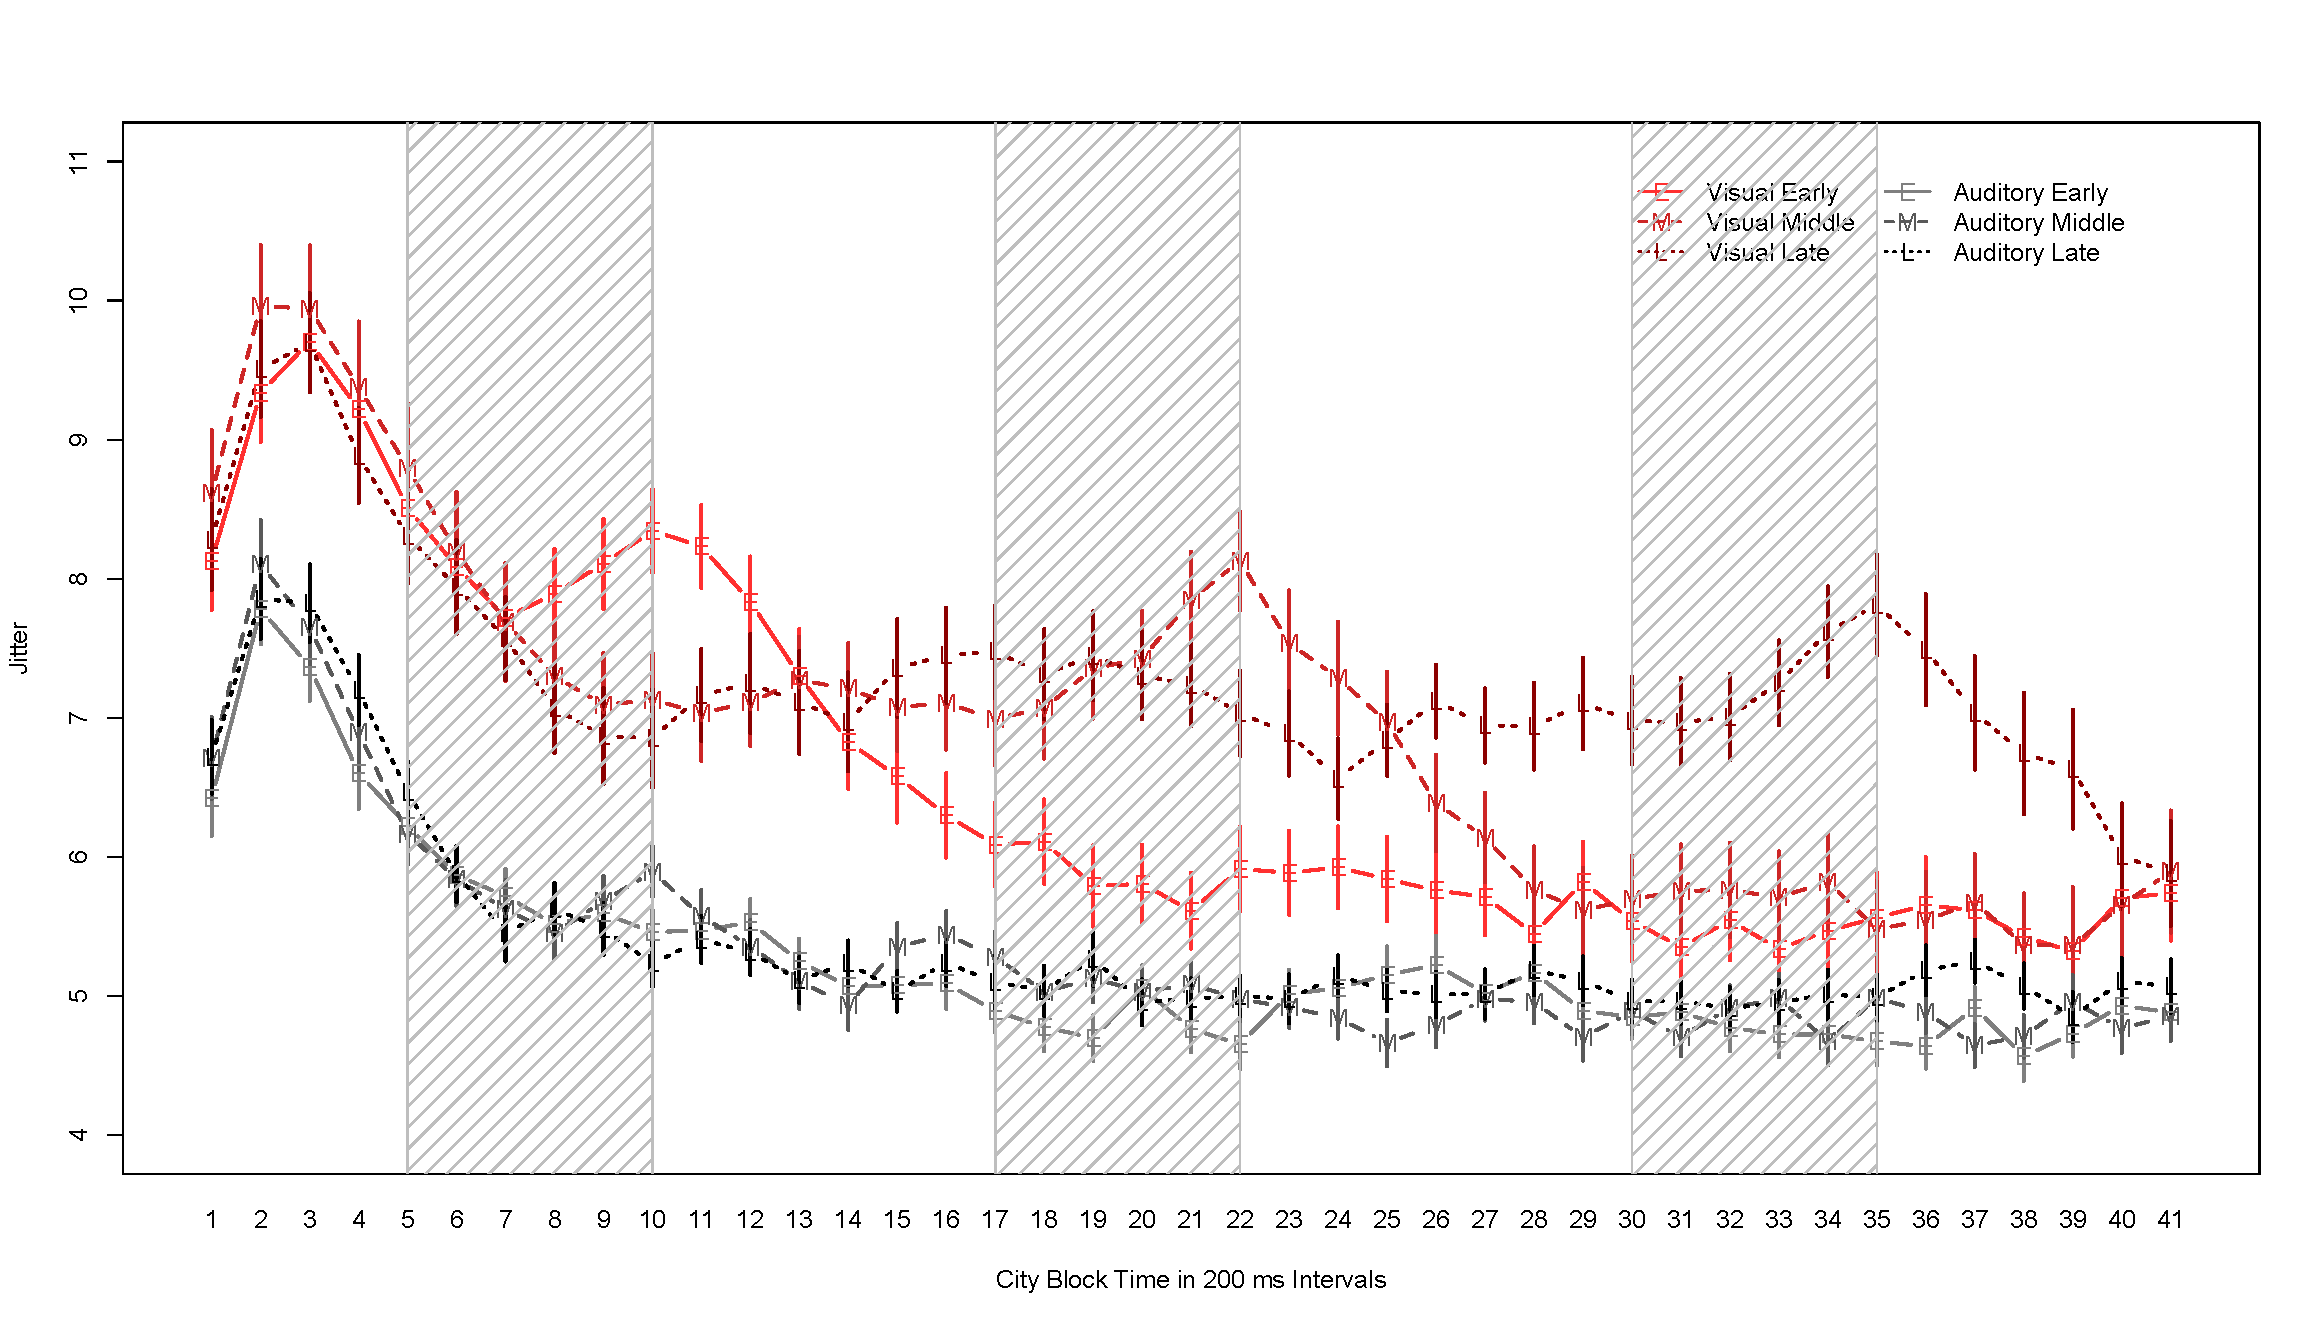
\includegraphics[width=.9\textwidth]{../zNvBkFigs/Rplot-e1jit41-best-110730}
	\end{figure}
\end{frame}

\begin{frame} 
	\frametitle{E1 RESULTS: Jitter by Condition - interesting because \dots}
	\begin{itemize}
		\item Being \emph{brain-bound} MRT would expect the greatest modality related difference to occur \alert{after} the new instruction appeared
		\item At that time people must process the visual or auditory information, delete one item from their old list of three turns, add a new item to the list, and begin rehearsing the new list
		\pause
		\item However, our data show the biggest differences are \alert{before} the new instruction appears

	\end{itemize}
\end{frame}

\begin{frame} 
	\frametitle{E1 RESULTS: Attention Shifts -- Fixations to the Arrow}
	\begin{figure}
		\centering
		\includegraphics[width=.9\textwidth]{../zNvBkFigs/Rplot_e1AttShftsToArrow}
		\begin{itemize}
			\item Main Effect of Condition
			\item No Significant differences involving Block or its interactions
			\item Interaction of Condition by Direction Interval is significant
		\end{itemize}

	\end{figure}
\end{frame}

\begin{frame}
	\frametitle{E1: DISCUSSION}
	\begin{itemize}
		\item As expected by MRT and FRF there is a significant difference between modality conditions for both \emph{Turn Accuracy} and \emph{Jitter}
		\item However, the details of the jitter data show the worse performance \emph{before} not \emph{after} the turn instruction is presented
		\item This implies that the processing of the new instruction, including the updating of the n-back style list of 3 items does not differ by modality
	\end{itemize}
Is this evidence that the \emph{cognitive control} is itself resource bound? {Wouldn't seem too surprisely if so.} \onslide<2->Or does this reflect low-level strategic changes in the selection of microprocedures used in this task? \onslide<3->Or are there other options we have not considered?
\end{frame}


%%% EXPERIMENT 2
\subsection{Experiment 2}
%%% EXPERIMENT 2


\begin{frame} 
	\frametitle{EXPERIMENT 2}
	\begin{itemize}
		\item Part of a longer study with 6 conditions
		\begin{itemize}
			\item Only two of the conditions will be discussed today
		\end{itemize}
		\item High vs Low Memory Load 
		\begin{itemize}
			\item High Load (HiMem) condition is identical to the Visual condition in E1
			\item Low Load (LoMem) condition is nearly identical to the High Load except Ss only need to remember one (1) instruction 
		\end{itemize}
		\item Basically the HiMem condition is identical to the Visual condition in E1. The LoMem condition is also identical with one exception; namely, LoMem is a \alert{n-back} of \alert{1} and not 3-back.
  	\end{itemize}
\end{frame}

\begin{frame}
	\frametitle{E2: RESULTS: Turn Accuracy by Condition}
	\vspace{-1.25cm}
	\begin{figure}
		\centering
		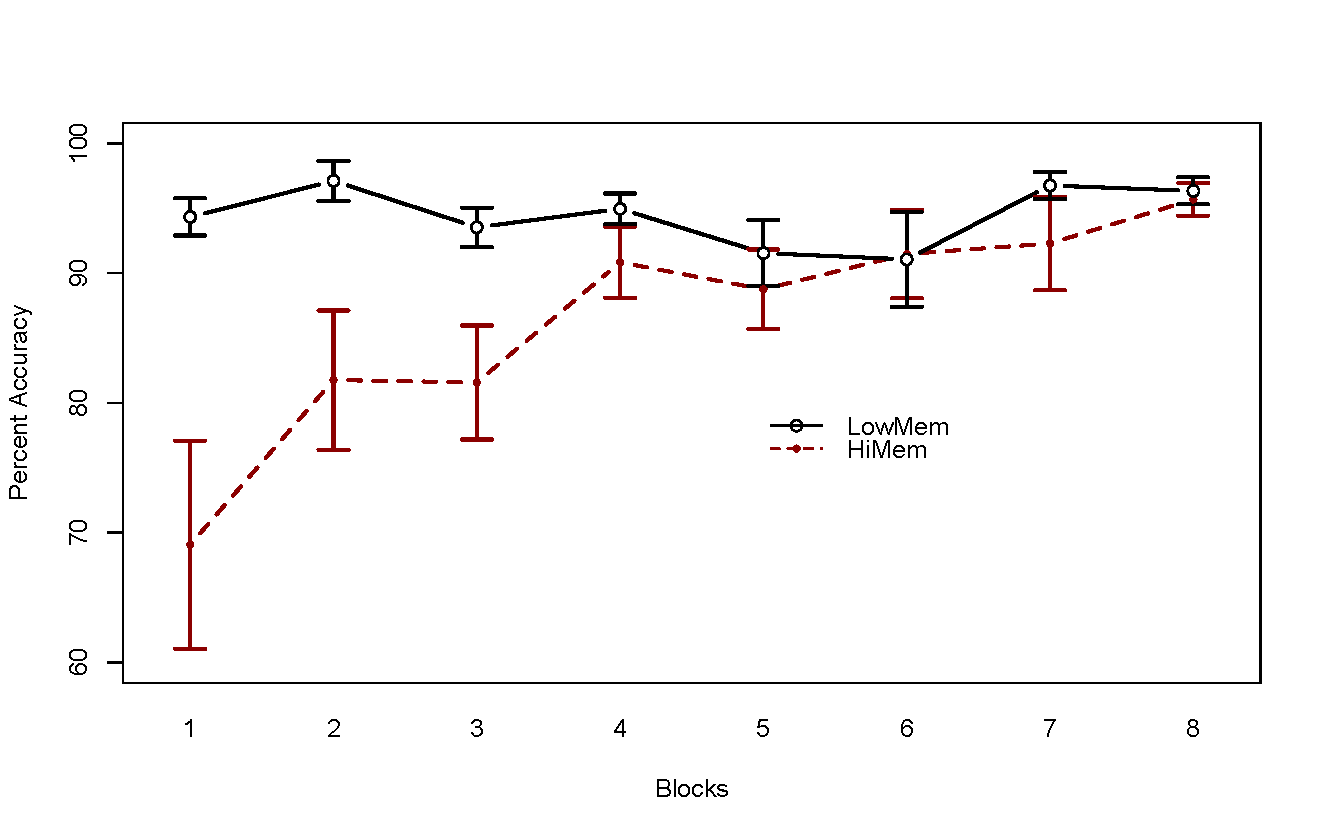
\includegraphics[width=.9\textwidth]{../zNvBkFigs/Rplot-E2Acc-LineChrt}
	\end{figure}
\end{frame}

\begin{frame} %[shrink=2]
	\frametitle{E2 RESULTS: Jitter by Condition}
	\vspace{-1cm}
	\begin{figure}
		\centering
		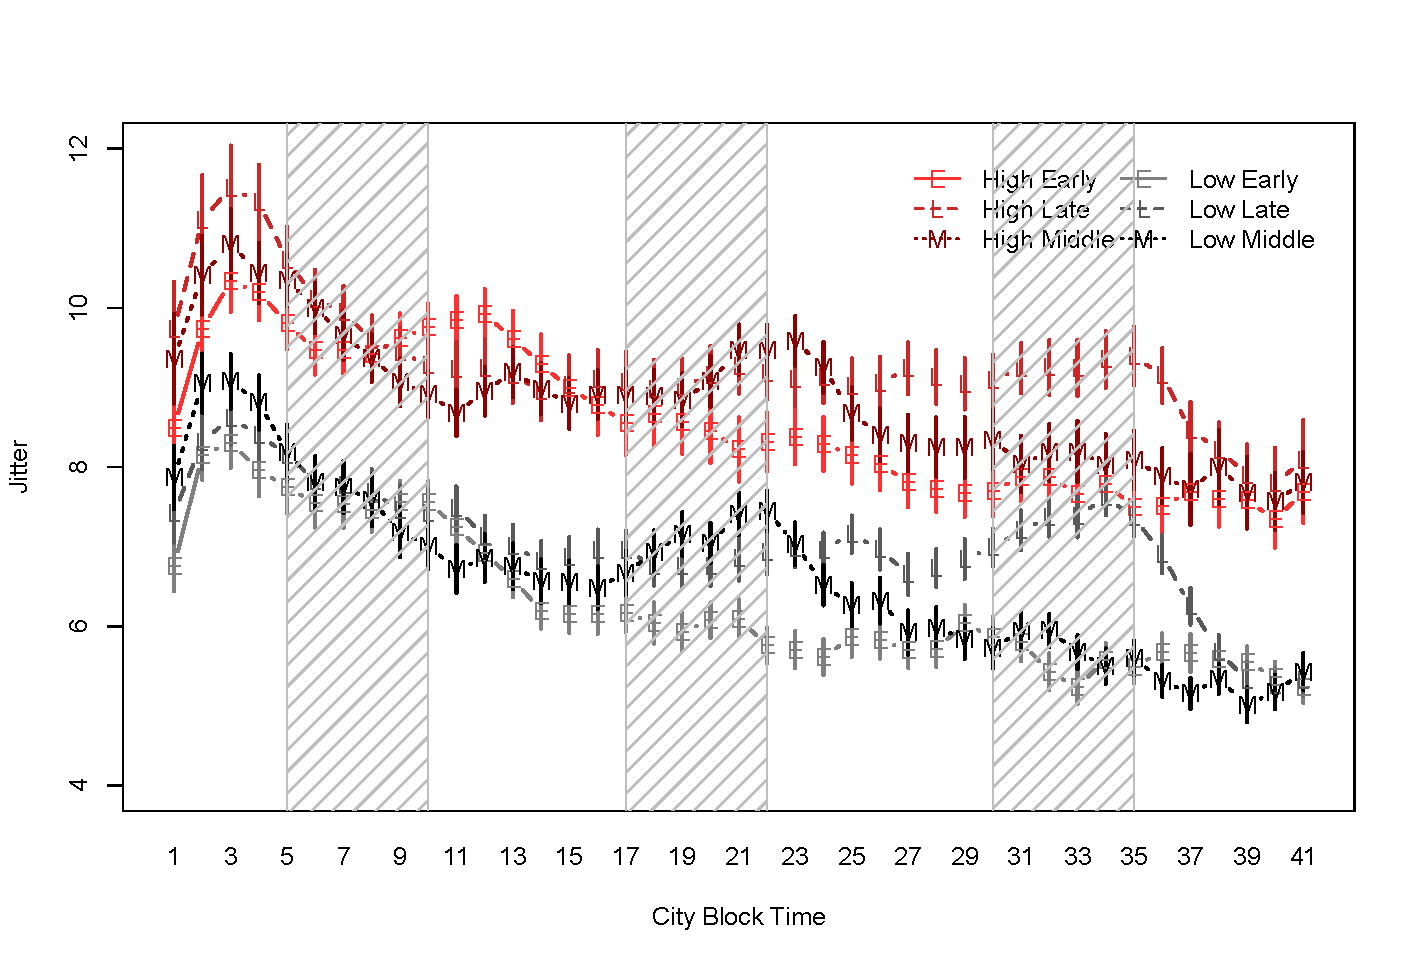
\includegraphics[width=.9\textwidth]{../zNvBkFigs/Rplot-E2-Jit41-noTit}
		{\tiny{\begin{itemize}
			\item Main Effect of Condition
			\item No Significant differences involving Block or its interactions
			\item Interaction of Condition by Direction Interval is significant
		\end{itemize}}}
	\end{figure}
\end{frame}

\begin{frame} 
	\frametitle{E2 RESULTS: Fixation Areas}
	\begin{figure}
		\centering
		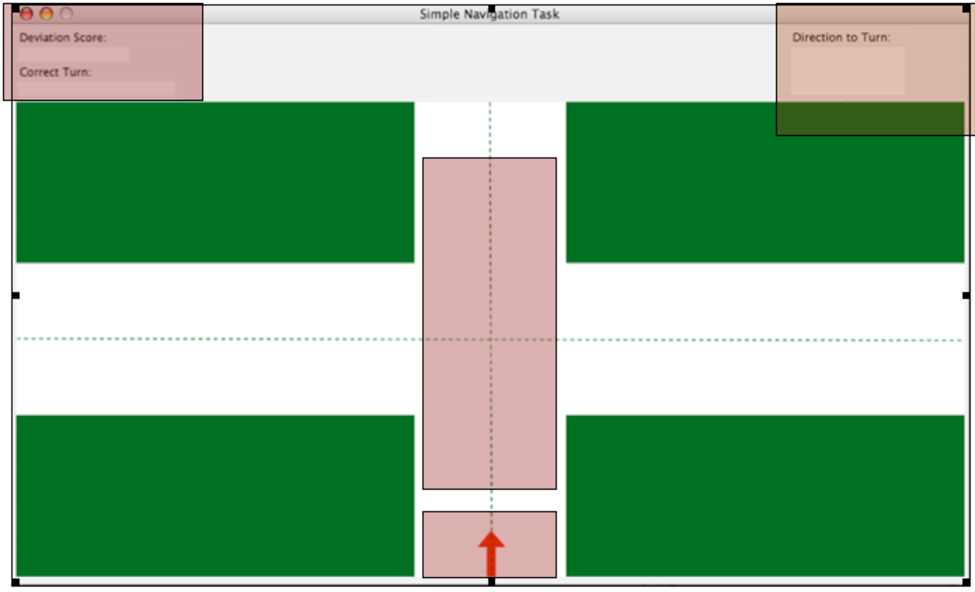
\includegraphics[width=.9\textwidth]{../zNvBkFigs/fig-E2-AOI}
	\end{figure}
\end{frame}

\begin{frame} 
	\frametitle{E2 RESULTS: Fixations by Area by Memory Load Condition}
	\vspace{-1cm}
	\begin{figure}
		\centering
		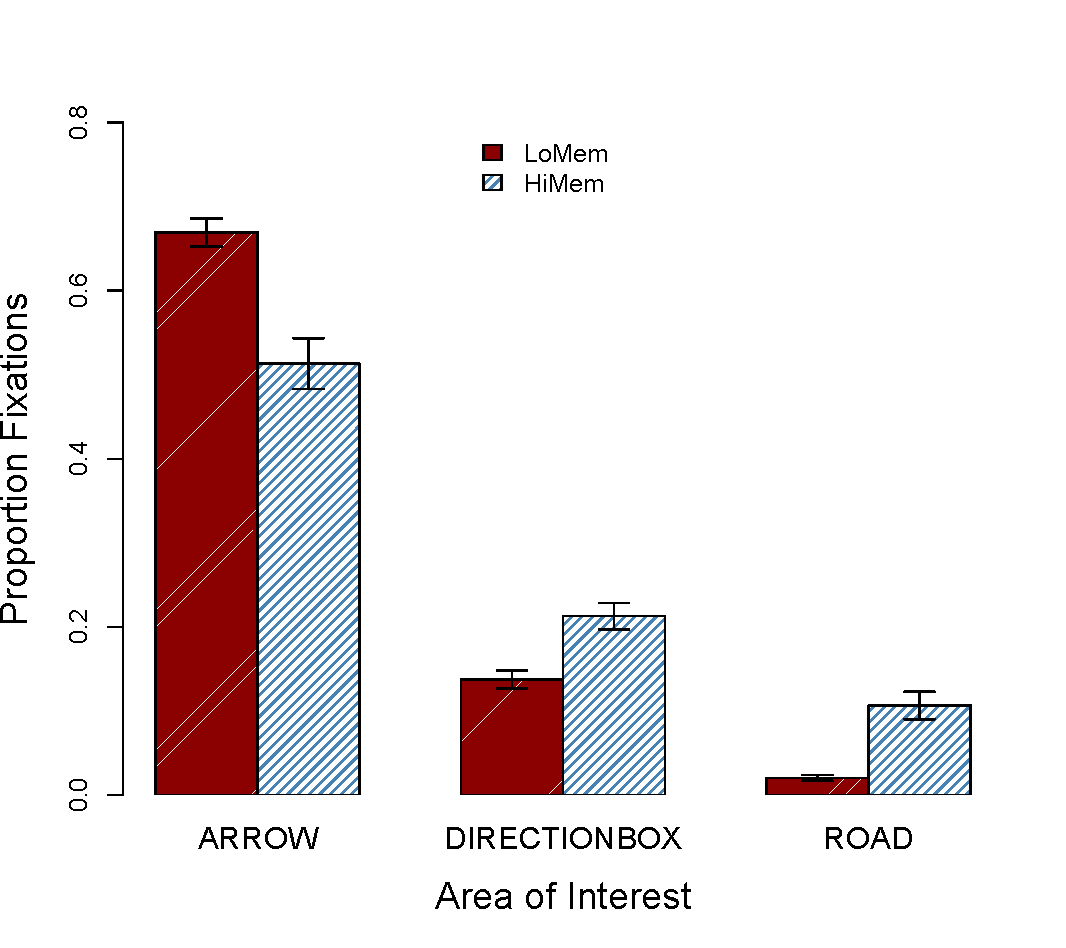
\includegraphics[width=.6\textwidth]{../zNvBkFigs/Rplot-E2-FixAoI}
	\end{figure}
	\vspace{-1cm}
	{\small{\begin{itemize}
		\item Memory x Area
	\end{itemize}}}

\end{frame}

\begin{frame} 
	\frametitle{E2 RESULTS: Fixations by Time}
	%\vspace{-1cm}
	  \begin{textblock}{2.5}(0,1)	
  		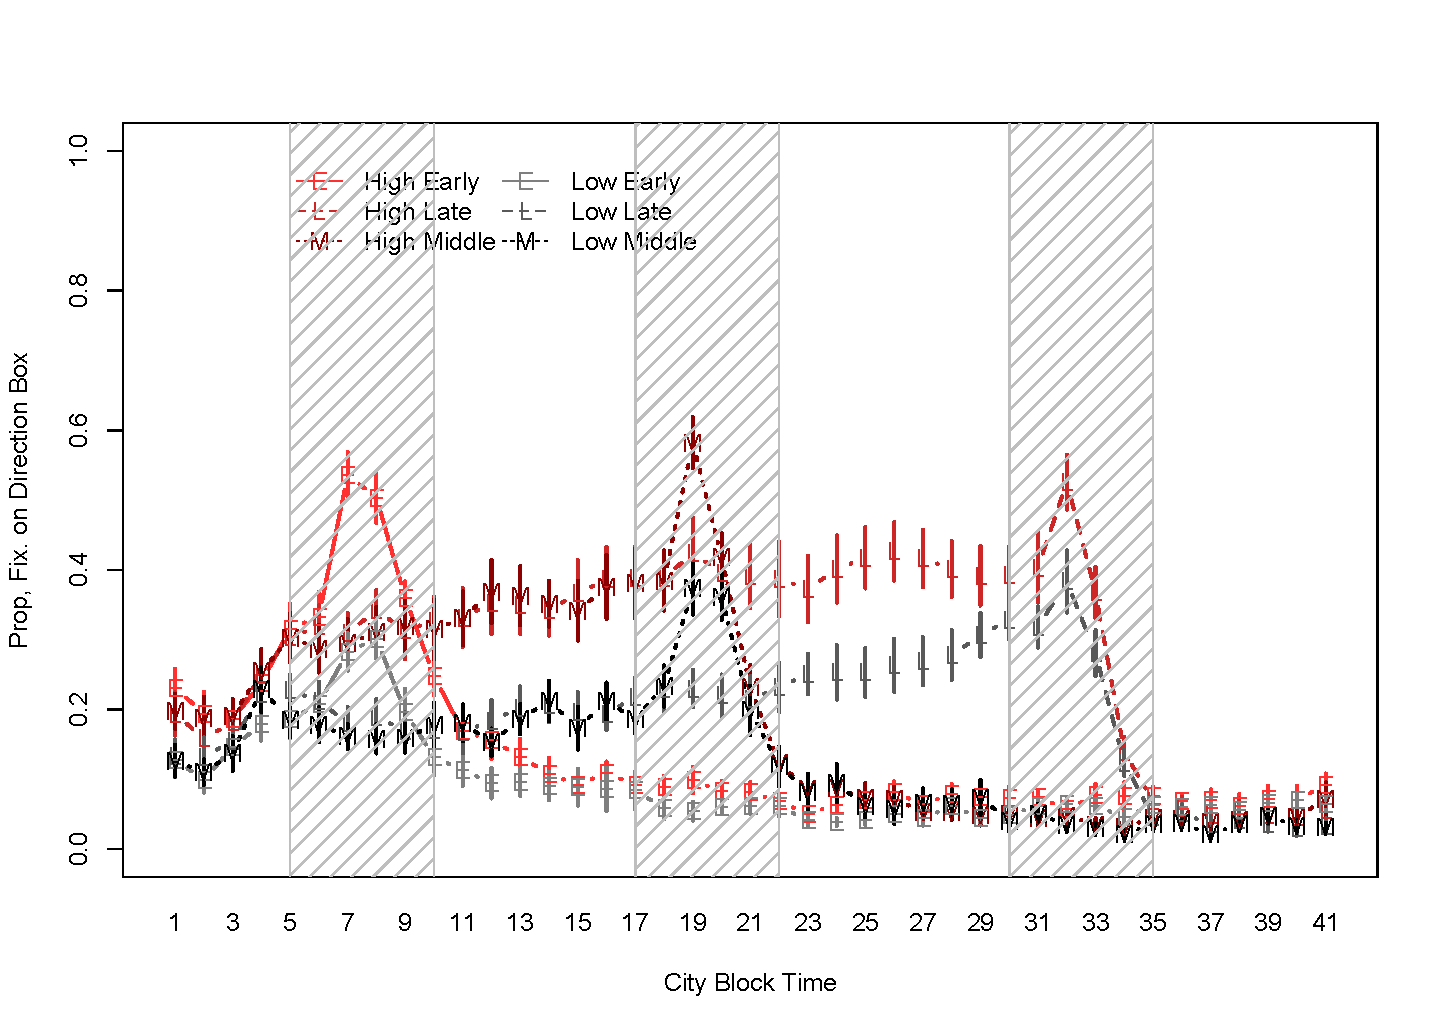
\includegraphics[scale=.3]{../zNvBkFigs/Rplot-E2-FixProp-DB-byCB}
    	   \end{textblock} 
	  \begin{textblock}{3}(0,7.5)	
  		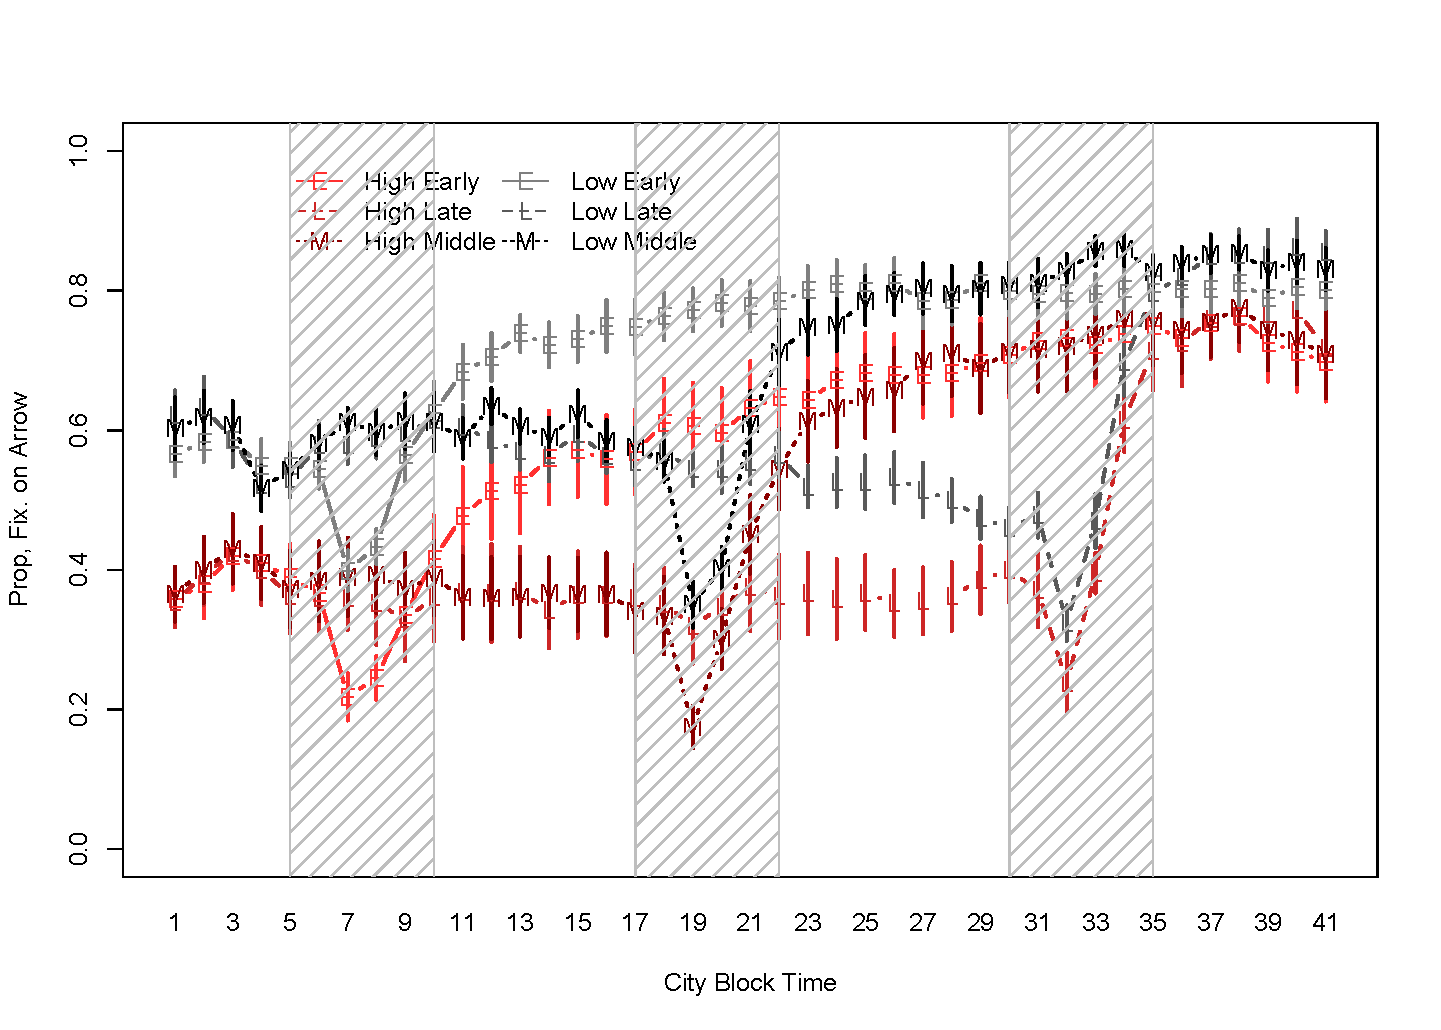
\includegraphics[scale=.3]{../zNvBkFigs/Rplot-E2-FixProp-Arrw-byCB}
    	   \end{textblock} 
		\begin{columns}
		\column{.6\textwidth}
		\column{.4\textwidth}
				 \small{Proportion of time spent fixating on the direction box (top) and arrow (bottom) for each of the three \emph{direction intervals}.  The gray area represents the time period when the instruction is on-screen.}
	\end{columns}
	\begin{textblock}{3}(5.5,2.5)	
		\color{wdgRed}{Direction Box}
    	\end{textblock} 
	\begin{textblock}{3}(5.5,14)	
		\color{wdgRed}{Arrow}
    	\end{textblock} 

\end{frame}


%%% stopped here last night
\begin{frame} 
	\frametitle{MORE DISPERSED EYE FIXATIONS}
	\begin{itemize}
		\item Is this a strategic difference? (\& consciously selected by our Subjects?)
		\pause
		\item Is this a pure resource consumption effect?
		\pause
		\item Or could it be a low-level change in microprocedures that reflect different priorities in these two task conditions??
 	\end{itemize}
\end{frame}

\begin{frame} 
	\frametitle{HOW DOES THIS STORY END??}
	\begin{itemize}
		\item We don't know
 	\end{itemize}
\end{frame}

\begin{frame} 
	\frametitle{STRATEGIC EFFECT??? (1)}
	Pro Argument \#1
	\begin{itemize}
		\item The penalty for getting an instruction wrong is much greater for the HiMem condition then the LoMem
		\item For example, getting instructions ordered wrong could mess up the score for several episodes
		\item In contrast, the LoMem group only has one instruction, doesn't have to worry about getting them ``messed up''. 
 	\end{itemize}
\end{frame}

\begin{frame} 
	\frametitle{STRATEGIC EFFECT??? (2)}
	Pro Argument \#2
		\begin{itemize}
		\item The greater difficulty of the Turn task for the HiMem group places more pressure on this group. Jitter seems fairly simple and they really do not know what is a good or bad jitter score
		\item But everyone would agree that keeping a list of three items in memory Is ``easy''
		\item Hence, forgetting something this ``simple'' leads people in this group to worry more about missing the instruction. Hence they monitor the direction box more and their performance on jitter suffers.
	\end{itemize}
\end{frame}

\begin{frame}
	\frametitle{CON ARGUMENT}
	\begin{itemize}
		\item ???
		\item Are resource limitations more reasonable? (Resource theories dominant applied work on cognitive workload and most discussions of basic work on control of cognition -- see \textcite{erik08pr.article} for a counterexception.
	\end{itemize}
\end{frame}



\againframe{4flaws}

\begin{frame}
	\includegraphics[width=\linewidth]{/Users/GrayMatter/Library/texmf/tex/zLogoFigs/cogWheels}
	\begin{textblock}{4}(11,7)
		\LARGE{\textcolor{wdgRed}{Thank You!!}}
	\end{textblock}
		
	%\begin{textblock}{5}(10,3)
	%	\LARGE{\textcolor{wdgRed}{Haben Sie vielen Dank!}}
	%\end{textblock}
\end{frame}

\begin{frame}[allowframebreaks]
	\frametitle{REFERENCES}
	\printbibliography
\end{frame}

\end{document}

